%%%%%%%%%%%%%%%%%%%%%%% file template.tex %%%%%%%%%%%%%%%%%%%%%%%%%
%
% This is a  template file for the LaTeX package SVJour3 width change file svepjc3.clo
% for Springer journal:
% The European Physical Journal C
%
% Copy it to a new file with a new name and use it as the basis
% for your article. Delete % signs as needed.
%
% This template includes a few options for different layouts and
% content for various journals. Please consult a previous issue of
% your journal as needed.
%
%%%%%%%%%%%%%%%%%%%%%%%%%%%%%%%%%%%%%%%%%%%%%%%%%%%%%%%%%%%%%%%%%%%
%
% First comes an example EPS file -- just ignore it and
% proceed on the \documentclass line
% your LaTeX will extract the file if required
%\begin{filecontents*}{example.eps}
%!PS-Adobe-3.0 EPSF-3.0
%%BoundingBox: 19 19 221 221
%%CreationDate: Mon Sep 29 1997
%%Creator: programmed by hand (JK)
%%EndComments
%gsave
%newpath
%  20 20 moveto
%  20 220 lineto
%  220 220 lineto
%  220 20 lineto
%closepath
%2 setlinewidth
%gsave
%  .4 setgray fill
%grestore
%stroke
%grestore
%\end{filecontents*}
%
%\RequirePackage{fix-cm}
%
\documentclass[twocolumn,epjc3]{svjour3}  
%
\smartqed  % flush right qed marks, e.g. at end of proof
%
% RP
% \RequirePackage{graphicx}
\RequirePackage[pdftex]{graphicx}
%
\RequirePackage{mathptmx}      % use Times fonts if available on your TeX system
%

% insert here the call for the packages your document requires
%\RequirePackage{latexsym}
%\RequirePackage[numbers,sort&compress]{natbib}
%\RequirePackage[colorlinks,citecolor=blue,urlcolor=blue,linkcolor=blue]{hyperref}
% etc.
%
% please place your own definitions here and don't use \def but
% \newcommand{}{}

\usepackage{amsmath,amssymb}
\usepackage[hypertexnames,setpagesize,%
    pdftex,%
    colorlinks,%
    citecolor=blue,%
    hyperindex,%
    plainpages=false,%
    bookmarksopen,%
    bookmarksnumbered%
  ]{hyperref}
% to turned off hypernation uncomment line below
%\usepackage[none]{hyphenat} 

% RP
% --- DO NOT remove this line:
\providecommand\texorpdfstring[2]{#1}
\usepackage[numbers,square,comma,sort&compress]{natbib}

\usepackage{textcomp}

% for displaying the line numbers:
\usepackage{lineno,xcolor}
\linenumbers
\setlength\linenumbersep{5pt}
\renewcommand\linenumberfont{\normalfont\tiny\sffamily\color{gray}}

% for TDM part
\def\kt{\ensuremath{k_t}}
\newcommand{\Pmax}{p}
\newcommand{\CCFM}{CCFMa,CCFMb,Catani:1989sg,CCFMd}


% for tikz pictures
\usepackage{tikz}
\usetikzlibrary{arrows,shapes,positioning}

% for tables
\usepackage{multirow}

\bibliographystyle{herafitter-epjc}


\usepackage{xspace}
%\newcommand\fitter{\mbox{\tt HERAFitter}}
\providecommand{\fitter}{{\texttt{HERAFitter}}\xspace}
\providecommand{\fastnlo}{{\texttt{fastNLO}}\xspace}
\providecommand{\applgrid}{{\texttt{APPLGRID}}\xspace}
\providecommand{\qcdnum}{{\texttt{QCDNUM}}\xspace}
\providecommand{\mcfm}{{\texttt{MCFM}}\xspace}
\providecommand{\nlojetpp}{{\texttt{NLOJet++}}\xspace}
\providecommand{\lhapdf}{{\texttt{LHAPDF}}\xspace}
\providecommand{\crundec}{{\texttt{CRunDec}}\xspace}
\providecommand{\hoppet}{{\texttt{HOPPET}}\xspace}
\providecommand{\GeV}{\ensuremath{\,\text{Ge\hspace{-.08em}V}}\xspace}
\providecommand{\pperp}{\ensuremath{p_{\perp}}\xspace}
\providecommand{\mur}{\ensuremath{\mu_\mathrm{R}}\xspace}
\providecommand{\muf}{\ensuremath{\mu_\mathrm{F}}\xspace}
\providecommand{\as}{\ensuremath{\alpha_\mathrm{s}}\xspace}
\providecommand{\asmz}{\ensuremath{\alpha_\mathrm{s}(M_Z)}\xspace}
\providecommand{\asq}{\ensuremath{\alpha_\mathrm{s}(Q)}\xspace}
\providecommand{\tmdlib}{{\texttt{TMDlib}}\xspace}


%
\journalname{Eur. Phys. J. C}
%
\begin{document}

\title{HERAFitter %\thanksref{t1}
}
\subtitle{Open Source QCD Fit Project \\
    { \small {Version 0.91 (svn 1458)}}
}

%\titlerunning{Short form of title}        % if too long for running head

% author list 
%\author{The \fitter Team\ref{alist}}
\author{%         HERAFitter developers team \and \\
%
S.~Alekhin$^{16,17}$\and
O.~Behnke$^{1}$\and
P.~Belov$^{1,12}$\and
M.~Botje$^{18}$\and
D.~Britzger$^{1}$\and
S.~Camarda$^{1}$\and 
A.M.~Cooper-Sarkar$^{2}$\and 
K.~Daum$^{30,31}$\and
C.~Diaconu$^{3}$\and 
J.~Feltesse$^{19}$\and
A.~Gizhko$^{1}$\and
A.~Glazov$^{1}$\and
A.~Guffanti$^{20}$\and
M.~Guzzi$^{1}$\and
F.~Hautmann$^{13,14,15}$\and
A.~Jung$^{32}$\and
H.~Jung$^{1,33}$\and
V.~Kolesnikov$^{4}$\and    
H.~Kowalski$^{1}$\and
O.~Kuprash$^{1}$\and
A.~Kusina$^{21}$\and
S.~Levonian$^{1}$\and
K.~Lipka$^{1}$\and
B.~Lobodzinski$^{29}$\and 
K.~Lohwasser$^{16}$\and
A.~Luszczak$^{5}$\and    
B.~Malaescu$^{25}$\and
R.~McNulty$^{28}$\and
V.~Myronenko$^{1}$\and
S.~Naumann-Emme$^{1}$\and
K.~Nowak$^{1}$\and
F.~Olness$^{21}$\and 
E.~Perez$^{23}$\and
H.~Pirumov$^{1}$\and
R.~Pla\v cakyt\. e$^{1}$\and
K.~Rabbertz$^{6}$\and    
V.~Radescu$^{1}$\and
R.~Sadykov$^{24}$\and
G.~Salam$^{26,27}$\and
A.~Sapronov$^{4}$\and
A.~Sch\"oning$^{10}$\and
T.~Sch\"orner-Sadenius$^{1}$\and
S.~Shushkevich$^{1}$\and    
W.~Slominski$^{7}$\and    
H.~Spiesberger$^{22}$\and
P.~Starovoitov$^{1}$\and    
M.~Sutton$^{8}$\and    
J.~Tomaszewska$^{9}$\and    
O.~Turkot$^{1}$\and
A.~Vargas$^{1}$\and
G.~Watt$^{11}$\and 
K.~Wichmann$^{1}$
%Karin Daum//R  
}
%\authorrunning{Short form of author list} % if too long for running head
\institute{$ $Deutsches Elektronen-Synchrotron (DESY), Hamburg, Germany\\
 $ ^{2}$ Department of Physics, University of Oxford, Oxford, United Kingdom \\
 $ ^{3}$ CPPM, IN2P3-CNRS, Univ. Mediterranee, Marseille, France \\
 $ ^{4}$ Joint Institute for Nuclear Research (JINR), Joliot-Curie 6, 141980, Dubna, Moscow Region, Russia \\
 $ ^{5}$ T. Kosciuszko Cracow University of Technology \\
 $ ^{6}$ Institut f\" ur Experimentelle Kernphysik, Karlsruhe, Germany \\
 $ ^{7}$ Jagiellonian University, Institute of Physics, Ul. Reymonta 4, PL-30-059 Cracow, Poland \\
 $ ^{8}$ University of Sussex, Department of Physics and Astronomy, Sussex House, Brighton BN1 9RH, United Kingdom \\
 $ ^{9}$ Warsaw University of Technology, Faculty of Physics, Koszykowa 75, 00-662 Warsaw, Poland \\
 $ ^{10}$ Physikalisches Institut, Universit\"at Heidelberg, Heidelberg, Germany \\
 $ ^{11}$ Institute for Particle Physics Phenomenology, Durham University, Durham, DH1 3LE, United Kingdom \\
 $ ^{12}$ Current address: Department of Physics, St. Petersburg State University, Ulyanovskaya 1, 198504 St. Petersburg, Russia\\
 $ ^{13}$ Dept. of Physics and Astronomy, University of Sussex, Brighton BN1 9QH, United Kingdom \\
 $ ^{14}$ Rutherford Appleton Laboratory, Chilton OX11 0QX, United Kingdom \\
 $ ^{15}$ Dept. of Theoretical Physics, University of Oxford, Oxford OX1 3NP, United Kingdom \\
 $ ^{16}$ Deutsches Elektronen-Synchrotron (DESY), Platanenallee 6, D–15738 Zeuthen, Germany \\
 $ ^{17}$ Institute for High Energy Physics,142281 Protvino, Moscow region, Russia \\
 $ ^{18}$ Nikhef, Science Park, Amsterdam, the Netherlands \\
 $ ^{19}$ CEA, DSM/Irfu, CE-Saclay, Gif-sur-Yvette, France \\
 $ ^{20}$ Niels Bohr Institute, University of Copenhagen, Denmark \\
 $ ^{21}$ Southern Methodist University, Dallas, Texas \\
 $ ^{22}$ PRISMA Cluster of Excellence, Institut f\"ur Physik (WA THEP), Johannes-Gutenberg-Universit\" at, D-55099 Mainz, Germany \\
 $ ^{23}$ CERN, European Organization for Nuclear Research, Geneva, Switzerland \\
 $ ^{24}$ Joint Institute for Nuclear Research, Joliot-Curie str. 6, Dubna, 141980, Russia \\ 
 $ ^{25}$ Laboratoire de Physique Nucl\' eaire et de Hautes Energies, UPMC and Universit\'e, Paris-Diderot and CNRS/IN2P3, Paris, France \\
 $ ^{26}$ CERN, PH-TH, CH-1211 Geneva 23, Switzerland \\
 $ ^{27}$ LPTHE; CNRS UMR 7589; UPMC Univ. Paris 6; Paris 75252, France \\
 $ ^{28}$ University College Dublin, Dublin 4, Ireland \\
 $ ^{29}$ Max Planck Institut F\"ur Physik, Werner Heisenberg Institut, F\"ohringer Ring 6, Mu\"nchen \\
 $ ^{30}$ Fachbereich C, Universit\"at Wuppertal, Wuppertal, Germany \\
 $ ^{31}$ Rechenzentrum, Universit\"at Wuppertal, Wuppertal, Germany \\
 $ ^{32}$ FERMILAB, Batavia, IL, 60510, USA \\
 $ ^{33}$ Elementaire Deeltjes Fysica, Universiteit Antwerpen, B 2020 Antwerpen, Belgium 
}
%

%
%
%\thankstext{t1}{Grants or other notes
%about the article that should go on the front page should be
%placed here. General acknowledgments should be placed at the end of the article.
%\thankstext{e1}{e-mail: fauthor@example.com}

%\authorrunning{Short form of author list} % if too long for running head

%\institute{Version 0.7 (svn 1383)
%\institute{Deutsches Elektronen-Synchrotron, DESY,
%            Notkestr. 85, 22607 Hamburg \label{addr1}
%           \and
%           Second address \label{addr2}
%           \and
%           \emph{Present Address:} if needed\label{addr3}
%}

\date{Received: date / Accepted: date}
% The correct dates will be entered by the editor


\setcounter{tocdepth}{4}
\maketitle

\begin{abstract}
\fitter \cite{herafitter:page} is an open-source package
which provides a framework for the determination of the
parton distribution functions (PDFs) of the proton and for
multifold analyses in Quantum Chromodynamics (QCD).

Measurements of lepton-proton deep inelastic scattering (DIS)
and of proton-proton (proton-antiproton) collisions
at hadron colliders are included in the \fitter package,
and are used to probe and constrain
the partonic content of the proton.

The partonic distributions are determined by using 
the factorisation properties of the hadronic cross sections 
in which short-distance perturbatively calculable hard scatterings      
and long-distance contributions that are the non-perturbative universal PDFs,
are factorised.

The \fitter platform provides a broad choice of options             
for the treatment of the experimental uncertainties and a common
environment where a large number of theoretical calculations and
methodological options are used to perform detailed QCD analyses.
The general structure of \fitter together with available methods
are described in this paper.

%The paper presents the \fitter package \cite{herafitter:page}
%which provides a framework for Quantum Chromodynamics (QCD) analyses related 
%to the proton structure.
%%in the context of multi-processes and multi-experiments.
%The main processes sensitive to the Parton Distribution Functions (PDFs) 
%of the proton are Deep-Inelastic-Scattering (DIS) 
%in $ep$ collisions at HERA and Drell-Yan (DY), jet and top quark production in 
%$pp$ ($p\bar{p}$) collisions at the LHC (Tevatron).
%Data of recent measurements are included into \fitter and can 
%be used for PDF determination
% based on the concept of the factorisable nature 
%of the cross sections of hard scattering measurements into process dependent 
%partonic scattering and universal PDFs.
%\fitter provides a comprehensive choice of options in the treatment of the experimental 
%data uncertainties, a large number of theoretical and methodological options 
%through interfaces to external software packages which are described here.
%
\keywords{PDFs \and QCD \and Fit \and proton structure}
% \PACS{PACS code1 \and PACS code2 \and more}
% \subclass{MSC code1 \and MSC code2 \and more}
\end{abstract}
   

\tableofcontents
            

\section{Introduction}
\label{sec:intro}
%\normalsize
In the era of the Higgs discovery and extensive searches
for signals of new physics at the LHC it is crucial
to have accurate Standard Model (SM) predictions for
hard scattering processes at the LHC.
The most common approach to calculate the SM cross sections for  
such reactions is to use collinear factorisation in perturbative QCD (pQCD):
%is with perturbative QCD using a (collinear) factorisation approach: 
%{\small
\begin{equation}
\small
\begin{array}{lcl}
\sigma^{pp\rightarrow H + X}(\alpha_s,\mu_r,\mu_f) & = &
\sum\limits_{a,b}\,  \int\limits_{0}\limits^{1} dx_1 \int\limits_{0}\limits^{1} dx_2\, f_a(x_1,\alpha_s,\mu_F) 
 f_b(x_2,\alpha_s,\mu_F)\\ 
& \times & \, \hat{\sigma}^{ab \rightarrow H + X}(x_1,x_2;\alpha_s,\mu_R,\mu_F).
%\sigma^{pp\rightarrow H + X}(\alpha_s,\mu_r,\mu_f) = 
%\sum_{a,b} \int_{0}^{1} dx_1 \int_{0}^{1} dx_2 f_a(x_1) 
% f_b(x_1,\alpha_s,\mu_F) \times \hat{\sigma}^{ab \rightarrow H + X}(x_1,x_2;\alpha_s,\mu_R,\mu_F)
\label{eq:fact}
\end{array}
\end{equation}
%}
Here the cross section $\sigma^{pp\rightarrow H + X}$ for inclusive
Higgs production is expressed
as a convolution of Parton Distribution Functions (PDF) $f_a$ and $f_b$
with the partonic cross section
% that describe
%the 
$\hat{\sigma}^{ab \rightarrow H + X}$.
%
The PDFs describe 
the probability of finding a specific parton $a$ ($b$) in the first (second) proton carrying a fraction $x_1$ ($x_2$) of its momentum.
%
The sum over indices $a$ and $b$ in Eq.~\ref{eq:fact} indicates the various 
kinds of partons,
i.e. gluons and quarks and antiquarks of different flavours, 
that are considered
as the constituents of the proton.
%
Both the PDFs and the partonic cross section depend on the strong coupling
constant $\alpha_s$, and the factorisation and renormalisation scales,
$\mu_F$ and $\mu_R$, respectively.
%
The partonic cross sections are calculable in pQCD, but
the PDFs cannot yet be predicted in QCD, they must rather be 
determined from measuement. They are assumed 
to be universal such that different scattering reactions can be used 
to constrain them; in particular one can use specific reaction data 
for determining the PDFs and then use these PDFs for
predicting other processes.
% via Eq.~\ref{eq:fact}.
%

The Deep Inelastic Scattering (DIS) data from the $ep$ collider HERA provides crucial information for determining the PDFs.
%
For instance, the gluon density relevant
for calculating the dominant gluon-gluon fusion contribution to the Higgs production
at the LHC can be accurately determined from the HERA data alone.
%
%Despite being often plagued by larger perturbative uncertainties,
Specific data from the Tevatron $p\bar{p}$ and the LHC $pp$ collider
can help to further constrain the PDFs.
%
The most sensitive processes at the  colliders are
Drell Yan production, W and Z asymmetries, associated production of W or Z boson 
and heavy quarks, top quark production and jet production.
%

\fitter represents a QCD analysis framework that aims at 
determining precise PDFs by integrating all the PDF sensitive information
from HERA, the Tevatron and the LHC.
%
The processes that are currently included in \fitter framework are listed in Tab.~\ref{tab:proc}.
%
\begin{table}
\small
%\tiny
\scriptsize

\begin{tabular}{|l|l|l|l|}
\hline
Data &Type &  Reaction & Theory      \\
        &     &     & calculation \\
\hline

HERA &DIS NC   &$ep\to ep$ & QCDNUM, RT, ACOT \\
HERA &DIS CC   &$ep\to \nu_e p$ & QCDNUM, RT, ACOT\\
HERA &DIS jets &$ep\to eX$ & FastNLO (NLOJet++)\\
HERA &DIS heavy quark & $ep\to ep $& ZM (QCDNUM), RT, ACOT, \\
     &                     &            & FFNS (ABM,QCDNUM) \\
\hline
Fixed Target &DIS NC   &$ep\to ep$ & ZM (QCDNUM), RT, ACOT \\
\hline
Tevatron, LHC &Drell Yan &$pp(\bar p)$ & APPLGRID (MCFM) \\
Tevatron, LHC &W charge asym &$pp(\bar p)$ & APPLGRID (MCFM) \\
Tevatron, LHC &top &$pp(\bar p)$ & APPLGRID (MCFM),  \\
              &    &             & HATHOR \\
Tevatron, LHC &jets &$pp(\bar p)$ & APPLGRID (NLOJet++) \\
                &  & & FastNLO (NLOJet++) \\
LHC&  DY+heavy quark &$pp(\bar p)$ & APPLGRID (MCFM) \\
\hline
\end{tabular}
\caption{The list of processes available in the \fitter package. {\bf you need references for the theory predictions in this caption}}
\label{tab:proc}
\end{table}
%
\normalsize
The basic functionality of HERAFitter is shown in Fig.~\ref{fig:flow} and consists of four parts: %{\bf needs to update figure!}
\begin{figure}[!ht]
   \centering
   \includegraphics[width=8cm]{flow.pdf}
   \caption{Schematic structure of the \fitter program.} 
 \label{fig:flow}
\end{figure}
\begin{description}
\item 
\bf {Input data:} \rm  All relevant cross section data from the various reactions
are stored internally in \fitter with the full information on their uncorrelated and correlated
uncertainties.
\item
\bf{Theory predictions:} \rm Predictions are obtained relying on the factorisation approach (Eq.~\ref{eq:fact}). PDFs are parametrised at a starting scale $Q_0$  by a chosen functional form with a set of free parameters $\vec{p}$. They are then evolved from $Q_0$ to the scale of the measurement using the 
Dokshitzer-Gribov-Lipatov-Altarelli-Parisi 
(DGLAP)~\cite{Gribov:1972ri, Gribov:1972rt, Lipatov:1974qm,
Dokshitzer:1977sg, Altarelli:1977zs} evolution equations 
as implemented in QCDNUM~\cite{qcdnum}, 
and then convoluted (Eq.~\ref{eq:fact}) with the hard parton cross sections calculated by
a specific theory program (as listed in Tab.~\ref{tab:proc}).
\item
\bf{Minimization:} \rm  PDFs are extracted from a least square fit by constructing a 
$\chi^2$ from the input data and the theory prediction.
The $\chi^2$ is  minimized iteratively 
with respect to the PDF parameters using the MINUIT\cite{minuit} program.
%
%Fitted values of $\vec{p}$ and estimated uncertainties are obtained.
%The fitted parameters $\vec(p)$ and obtained from the uncertainties of the parameters are determined (from chi2+1???)
%
\item
\bf{Results:} \rm  The fitted parameters $\vec{p}$ and their estimated uncertainties are produced.
The resulting PDFs are provided in a format ready to be used by the LHAPDF 
library. Tools are supplied which allow the PDFs to be
graphically 
displayed at arbitrary scales with their one sigma uncertainty bands.
To demonstrate the fit consistency, plots 
which compare the input data to the fitted theory predictions can be made using
tools supplied with the package. 
This is illustrated in the Fig.~\ref{fig:data} showing  
HERA~I data (the default data set in \fitter) compared to predictions based on 
HERAPDF1.0\cite{h1zeus:2009wt}. This figure also illustrates this comparison 
taking into account the systematic uncertainty shift parameters which are 
applied to the predictions in the nuisance parameter method of accounting for 
correlated systematic uncertainties (see section~\ref{sec:chi2representation}) and the pulls 
{\bf you need to define exactly what you mean by a pull here, don't just leave it in the figure caption}.
\begin{figure}[!ht]
   \centering
   \includegraphics[width=8cm]{datatheory.pdf}
   \caption{An illustration of the \fitter drawing tools comparing the measurements (in this case HERA I) to the predictions of the fit. In addition, ratio plots are also provided together with the pull distribution (right panel).} 
 \label{fig:data}
\end{figure}

\end{description}
%
%This paper provides a comprehensive description of  \\
%the \fitter\ package.
%which is designed for analysis of the High Energy Physics data.
%The package has been developed by members of the H1 and ZEUS collaborations
%with an exclusive support of different theoretical groups.
%The main purpose of the \fitter\ package is analysis of the 
%data from the $e^{\pm}p$, $p\bar{p}$, and $pp$ collider experiments
%information obtained from the deep inelastic scattering experiments
%and the determination of the parton density functions (PDFs).
%The broad range of data taken from the $e^{\pm}p$, $p\bar{p}$, and $pp$ collider experiments can be
%studied by the package. 

%Based on the concept of factorisable nature of the cross sections into universal parton distribution functions (PDFs) and process dependent partonic scattering cross sections, 

The \fitter\ program facilitates the determination of the PDFs from many 
cross section measurements at $ep$, $p\bar{p}$ or $pp$ colliders.  
 It includes various options for theoretical calculations and various choices 
of how to 
account for the experimental uncertainties. Therefore, this project represents 
an ideal environment for benchmarking studies and a unique platform for the QCD interpretation of analyses within the LHC experiments,
as already demonstrated by several publicly available results using the \fitter\ 
framework~\cite{atlas:strange,atlas:jets,atlas:hm,cms:strange,cms:jets,h1:2012kk,h1zeus:charm}.  

The outline of this paper is as follows.
%
Section~\ref{sec:theory} discusses the various processes 
and corresponding theoretical calculations performed in the DGLAP~\cite{Gribov:1972ri,Gribov:1972rt,Lipatov:1974qm,
Dokshitzer:1977sg,Altarelli:1977zs} formalism that are available in \fitter.
Alternative approaches to the DGLAP formalism are presented in section~\ref{sec:alternative}.
%
In section~\ref{sec:techniques} various different choices made in the 
theory calculations are described.
Section~\ref{sec:method} elucidates the 
methodology of determining PDFs through fits based on various
% {\bf (what do you mean here
%by approaches?)} 
 $\chi^2$ definitions used in the
minimisation procedure. 
%
Specific applications of the package are given in
section ~\ref{sec:examples}. 
%
%{\bf add something more here?.}

\section{HERAFitter Structure}
%
\label{sec:structure}

\fitter is a flexible open-source platform for the QCD analyses of different experimental measurements, 
providing a versatile environment for benchmarking studies. It is widely used within 
LHC experiments~\cite{atlas:strange,atlas:jets,atlas:hm,cms:strange,cms:jets,h1:2012kk,h1zeus:charm}.  

The functionality of \fitter is schematically illustrated in Fig.~\ref{fig:flow} and it can be divided in four main blocks: %{\bf needs to update figure!}
\begin{figure}[!ht]
  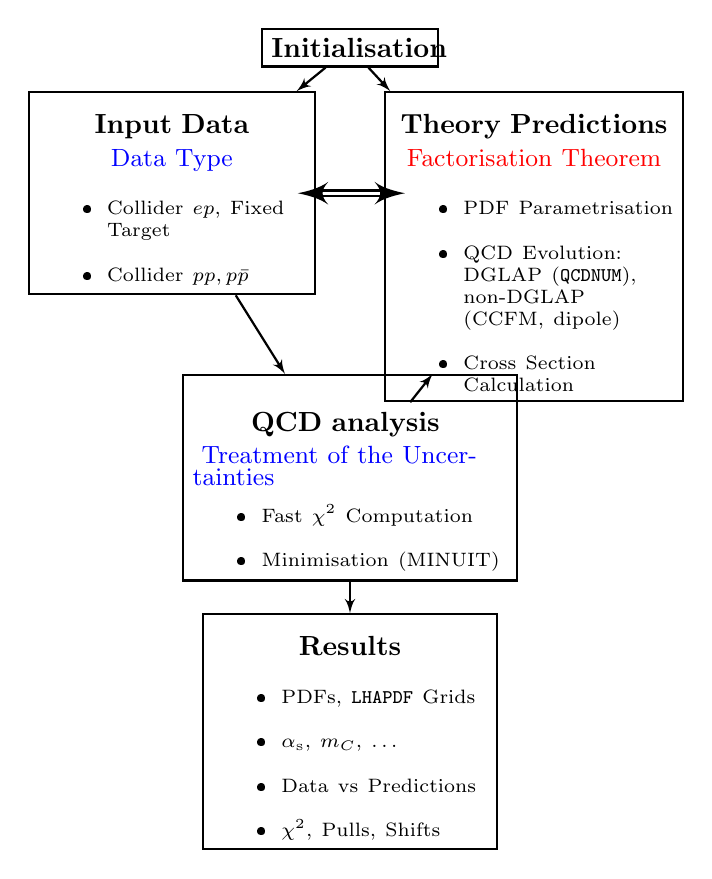
\begin{tikzpicture}[node distance=1cm, auto,>=latex', thick]
%      \path[->] node[draw, text width=2cm, align=center] at (0,0) (init) {\bf Initialization};
      \path[->] node[draw, text width=2cm, text centered] at (0,0) (init) {\bf Initialisation};
      \path[->] node[draw, below left=0.3cm and -0.7cm of init, text width=3.4cm] (data) 
                    {\begin{center} \vspace{-0.3cm}{\bf Input Data} 
		      \\ {\color{blue}\small Data Type} 
		     \end{center} 
		     {\scriptsize 
		     \begin{itemize}
                      \vspace{-0.3cm}
		      \item Collider $ep$, Fixed Target
		      \item Collider $pp, p\bar p$
		     \end{itemize}}
		     } (init) edge (data);
      \path[->] node[draw, below right=0.3cm and -0.7cm of init, text width=3.55cm] (theory) 
                    {\begin{center} \vspace{-0.3cm}{\bf Theory Predictions} 
		      \\ {\color{red}\small Factorisation Theorem} 
		     \end{center} 
		     {\scriptsize 
		     \begin{itemize}
                      \vspace{-0.3cm}
		      \item PDF Parametrisation
              \item QCD Evolution:  \\
                   DGLAP (\qcdnum), non-DGLAP (CCFM, dipole)
		      \item Cross Section Calculation
		     \end{itemize}}
		     } (init) edge (theory);
      \path[->] node[draw, below right=1.0cm and -1.7cm of data, text width=4cm] (minuit) 
                    {\begin{center} \vspace{-0.1cm}{\bf QCD analysis} 
                      \vspace{-0.2cm}
		     \end{center} 
		     {\color{blue}\small \ Treatment of the Uncertainties} 
		     {\scriptsize 
                      \vspace{-0.1cm}
		     \begin{itemize}
             \item Fast $\chi^2$ Computation 
             \item Minimisation (MINUIT)
		     \end{itemize}}
		     } (data) edge (minuit)
		     (theory) edge (minuit)
		     (data) ++ (1.6,0) edge [<->,double equal sign distance] ++(1.36,0) (theory);
      \path[->] node[draw, below =0.4cm  of minuit, text width=3.5cm] (res) 
                    {\begin{center} \vspace{-0.3cm}{\bf Results} 
		     \end{center} 
		     {\scriptsize 
		     \begin{itemize}
                      \vspace{-0.3cm}
		      \item PDFs, \lhapdf Grids
		      \item \as, $m_C$, \dots
		      \item Data vs Predictions
		      \item \(\chi^2\), Pulls, Shifts
		     \end{itemize}}
		     } (minuit) edge (res);
  \end{tikzpicture}
  \caption{Schematic structure of the \fitter program.} 
  \label{fig:flow}
\end{figure}

%\begin{figure}[!ht]
%   \centering
%   \includegraphics[width=8cm]{flow.pdf}
%   \caption{Schematic structure of the \fitter~program.} 
% \label{fig:flow}
%\end{figure}
\begin{description}
\item 
\bf {Input data:} \rm Different available measurements from the various processes
are implemented in the \fitter package including the full information on their uncorrelated 
and correlated uncertainties. HERA data 
are sensitive to light quark and gluon densities mostly through scaling violations, 
covering low and medium $x$ ranges. These data are the basis of any proton PDF extraction,
and are used by all global PDF groups \cite{MSTWpdf, CT10pdf, NNPDFpdf, ABMpdf, JRpdf}. 
However, improvements in precision of PDFs require additional constraints on the gluon and 
quark distributions at high-$x$, better understanding of heavy quark distributions and 
decomposition of the light-quark sea.  For these purposes, the measurements of the fixed-target 
experiments, Tevatron and LHC are of particular importance.
%
%Additional measurements provide constraints to the sea flavour decomposition, such as the new 
%results from the LHC, as well as constraints to PDFs in the kinematic phase-space regions 
%where HERA data is not measured precisely, such as the high $x$ region for the gluon and valence 
%quark distributions from Tevatron and fixed target experiments.
%
The processes that are currently available in \fitter framework are listed in Tab.~\ref{tab:proc}.

%
\begin{table}
\small
%\tiny
\scriptsize

\begin{tabular}{|l|l|l|l|}
\hline 
\textbf{Data} &\textbf{Process}&\textbf{Reaction}&\textbf{Theory} \\
        &     &               &\textbf{calculations, schemes}  \\
\hline \hline \\ [-2.5ex]
%\multirow{6}{*}{HERA} &DIS NC   &$ep\to eX$      & TR', ACOT \\
HERA &DIS NC   &$ep\to eX$      & TR', ACOT \\
     &         &                & ZM (\qcdnum) \\
     &         &                & FFN (\texttt{OPENQCDRAD}, \\
     &         &                & \qcdnum), \\ 
     &         &                & TMD (uPDFevolv) \\ [0.5ex]
\cline{2-4}  \\ [-2.0ex]
     &DIS CC   &$ep\to \nu_e X$ & ACOT, ZM (\qcdnum) \\
     &         &                & FFN (\texttt{OPENQCDRAD)} \\  [0.5ex]
\cline{2-4}  \\ [-2.0ex]
     &DIS jets &$ep\to e\ \mathrm{jets}$      & \nlojetpp (\fastnlo)\\ [0.5ex]
\cline{2-4} \\ [-2.0ex]
     &DIS heavy quarks & $ep\to e c \bar{c} X$, & ZM (\qcdnum), \\
     &         & $ep\to e b \bar{b} X$ & TR', ACOT, \\
     &         &                & FFN (\texttt{OPENQCDRAD}, \\
     &         &                & \qcdnum) \\  [0.5ex]
\hline \\ [-2.5ex]
Fixed Target   &DIS NC          &$ep\to eX$ & ZM (\qcdnum), \\
     &         &                & TR', ACOT, \\ [0.5ex]
     &         &                & FFN (\texttt{OPENQCDRAD}, \\
     &         &                & \qcdnum) \\  [0.5ex]
\hline \\ [-2.5ex]
Tevatron, LHC &Drell-Yan &$pp(\bar p)\to l\bar l X$, & \mcfm (\applgrid) \\
              &          &$pp(\bar p)\to l\nu  X$ &                 \\ [0.5ex]
\cline{2-4}  \\ [-2.0ex]
%Tevatron, LHC &W charge asym &$pp(\bar p) \to l\nu X$ & MCFM (\texttt{APPLGRID}) \\
%\hline
              &top pair   &$pp(\bar p) \to t\bar t X$  & \mcfm (\applgrid),  \\
              &            &                            & \texttt{HATHOR}      \\  [0.5ex] 
\cline{2-4}  \\ [-2.0ex]
              &single top &$pp(\bar p) \to t l \nu X$,      & \mcfm (\applgrid) \\
              &           &$pp(\bar p) \to tX$,             &  \\
              &           &$pp(\bar p) \to tWX$             &  \\ [0.5ex]
\cline{2-4}  \\ [-2.0ex]
             &jets &$pp(\bar p) \to \mathrm{jets} X$ & \nlojetpp (\applgrid), \\
                &  & & \nlojetpp (\fastnlo) \\ [0.5ex]
\hline  \\ [-2.5ex] 
LHC& DY+heavy quarks &$pp \to VhX$ & \mcfm (\applgrid) \\  [0.5ex]
\hline
\end{tabular}
\caption{The list of processes available in the \fitter package. 
The references for the individual calculations and their implementations are given in the text.
}
%The APPLGRID~\cite{Carli:2010rw} and FastNLO~\cite{Kluge:2006xs,Wobisch:2011ij,Britzger:2012bs} 
%techniques for the fast interface to theory calculations are described in section~\ref{sec:techniques}.} 
\label{tab:proc}
\end{table}
%
\normalsize
\item
\bf{Theory predictions:} \rm  Predictions for cross section of different processes are obtained using 
the factorisation approach (Eq.~\ref{eq:fact}). The PDFs are parametrised at a starting input scale $Q_0^2$  
by a chosen functional form with a set of free parameters $\vec{p}$. 
These PDFs are evolved to the scale of the measurement $Q^2$, $Q^2>Q_0^2$.
The evolution follows either DGLAP \cite{Gribov:1972ri, Gribov:1972rt, Lipatov:1974qm,
Dokshitzer:1977sg, Altarelli:1977zs} (as implemented in \qcdnum~\cite{qcdnum}), CCFM \cite{\CCFM} 
or dipole models~\cite{Golec-Biernat:1998js,Iancu:2003ge,Bartels:2002cj}.
The prediction of a particular process cross section is obtained by a convolution of the evolved 
PDFs and the partonic cross section, calculated at a certain order in QCD 
with a relevant theory program (as listed in Tab.~\ref{tab:proc}).
%from $Q_0^2$ to the scale of the measurement using the 
%Dokshitzer-Gribov-Lipatov-Altarelli-Parisi 
%(DGLAP)~\cite{Gribov:1972ri, Gribov:1972rt, Lipatov:1974qm,
%Dokshitzer:1977sg, Altarelli:1977zs} evolution equations 
%(as implemented in \qcdnum~\cite{qcdnum}), 
%CCFM \cite{\CCFM} or dipole models~\cite{Golec-Biernat:1998js,Iancu:2003ge,Bartels:2002cj} 
%and then convoluted with the hard parton cross sections calculated
%using a relevant theory program (as listed in Tab.~\ref{tab:proc}).
\item
\bf{QCD analysis:} \rm  
The PDFs are 
are determined by the least square fit, minimising the $\chi^2$ function with respect to $\vec{p}$
using the MINUIT~\cite{minuit} program.
%extracted from a least square fit by minimising the  $\chi^2$ function with respect to free parameters. 
%The $\chi^2$ function is formed from the input data and the theory prediction.
%The $\chi^2$ is  minimised iteratively 
%with respect to$\vec{p}$ using the MINUIT~\cite{minuit} program.
Various choices of accounting for the experimental uncertainties are employed in \fitter, either using 
a nuisance parameter method for the correlated systematic uncertainties, 
or a covariance matrix method as described in section~\ref{sec:chi2representation}). In addition, \fitter allows to study different statistics 
assumptions for the distributions of the systematic uncertainties i.e. Gauss~\cite{hera-lhc:report2009} (see section~\ref{sec:experimentalerrors}).
%
%In the $\chi^2$ minimisation,
%The parameters $\vec{p}$ of the parametrised PDFs and their uncertainties are extracted from the minimisation fit.
%Fitted values of $\vec{p}$ and estimated uncertainties are obtained.
%The fitted parameters $\vec(p)$ and obtained from the uncertainties of the parameters are determined (from chi2+1???)
%
\item
\bf{Results:} \rm 
%The fitted parameters $\vec{p}$ and their estimated uncertainties are produced. 
The resulting PDFs are provided in a format ready to be used by the \lhapdf 
library~\cite{lhapdf,lhapdfweb} (or by \tmdlib \cite{tmdlref}).
\fitter drawing tools can be used to display the PDFs with their uncertainties at a chosen scale.  
%Drawing tools are supplied which allow the PDFs to be
%graphically  displayed at chosen scales by the users with their one sigma uncertainty bands. 
As an example, a first set of PDFs extracted using \fitter from HERA I data, HERAPDF1.0 \cite{h1zeus:2009wt}, 
is shown in Fig.~\ref{fig:hera1}.
%%%Since then several other PDF sets were produced within the HERA \cite{hera:grids} and LHC \cite{atlas:grids} collaborations.
%In addition to the PDF display, 
The comparison of data used in the fit to the theory predictions are also produced. 
% plots which compare the input data to the fitted theory predictions can be produced 
%to demonstrate the fit consistency. 
\begin{figure}[!ht]
   \centering
   \includegraphics[width=8cm]{hera1.pdf}
   \caption{Distributions of valence ($xu_v$, $xd_v$), sea ($xS$) and the gluon ($g$) densities in HERAPDF1.0~\cite{h1zeus:2009wt}. 
       The gluon and the sea distributions are scaled down by a factor of 20.
       The experimental, model and parametrisation uncertainties are shown as colored bands.}
       %Summary plots of valence ($xu_v$, $xd_v$), total sea ($xS$, scaled) and gluon ($xg$, scaled) densities
       %with their experimental, model and parametrisation uncertainties shown as colored bands at the scale 
       %of $Q^2=10 \ \GeV^2$ for the HERAPDF1.0 PDF set~\cite{h1zeus:2009wt}.}
 \label{fig:hera1}
\end{figure}
%In Fig.~\ref{fig:data}, a comparison of inclusive NC data from the HERA~I running period with predictions based on HERAPDF1.0 is shown. 
The inclusive NC data from the HERA I are compared with the predictions based on 
HERAPDF1.0 PDFs in Fig.~\ref{fig:data}.

Also shown are theory predictions, obtained using the nuisance parameter method, 
which accounts for correlated systematic
shifts when using the nuisance parameter method that accounts for 
correlated systematic uncertainties. 
The consistency of the measurements and the theory is expressed by pulls, defined as a difference between data 
and theory divided by the uncorrelated error of the data. 
In each kinematic bin of the measurement, pulls are provided in units of sigma.  
%As an additional consistency check between data and the theory predictions, pull information, defined as the difference between data and prediction divided by the uncorrelated uncertainty of the data, is displayed in units of sigma shifts for each given data bin.
\begin{figure}[!ht]
   \centering
   \includegraphics[width=8.6cm]{datatheory.pdf}
   \caption{An illustration of the consistency of HERA measurements~\cite{h1zeus:2009wt} and the theory predictions, 
       obtained in \fitter with the default drawing tool.} 
       %In addition, ratio plots are also provided together with the pull distribution (right panel).}    
 \label{fig:data}
\end{figure}

\end{description}
%
%This paper provides a comprehensive description of  \\
%the \fitter\ package.
%which is designed for analysis of the High Energy Physics data.
%The package has been developed by members of the H1 and ZEUS collaborations
%with an exclusive support of different theoretical groups.
%The main purpose of the \fitter\ package is analysis of the 
%data from the $e^{\pm}p$, $p\bar{p}$, and $pp$ collider experiments
%information obtained from the deep inelastic scattering experiments
%and the determination of the parton density functions (PDFs).
%The broad range of data taken from the $e^{\pm}p$, $p\bar{p}$, and $pp$ collider experiments can be
%studied by the package. 

%Based on the concept of factorisable nature of the cross sections into universal parton distribution functions (PDFs) and process dependent partonic scattering cross sections, 

%The \fitter\ program facilitates the determination of the PDFs from many 
%cross section measurements at $ep$, $p\bar{p}$ or $pp$ colliders.  
% It includes various options for theoretical calculations and various choices 
%of how to 
%account for the experimental uncertainties. 
%The \fitter project provides a versatile environment for benchmarking studies 
%and a flexible platform for the QCD interpretation of analyses within the LHC experiments,
%as already demonstrated by several publicly available results using the \fitter 
%framework~\cite{atlas:strange,atlas:jets,atlas:hm,cms:strange,cms:jets,h1:2012kk,h1zeus:charm}.  

\section{Theoretical Input}
\label{sec:theory}


%The proton PDFs are classically extracted from QCD fits by a measure of 
%the agreement between experimental data and corresponding theory models.
%During the fit procedure in the \fitter\ framework, the PDFs are
%parametrised at a starting scale $Q^2_0$ chosen to be below the charm 
%mass threshold and then evolved using coupled, integro-differential
%Dokshitzer-Gribov-Lipatov-Altarelli-Parisi 
%(DGLAP)~\cite{Gribov:1972ri,Gribov:1972rt,Lipatov:1974qm,
%Dokshitzer:1977sg,Altarelli:1977zs} evolution equations 
%as implemented in the QCDNUM~\cite{qcdnum} program in the $\overline{\text{MS}}$ scheme. 
%The evolution can be performed in the LO, NLO or NNLO accuracy~\cite{Curci:1980uw,Furmanski:1980cm}.
%
In this section the theoretical formalism for various processes available in \fitter is described.
%The PDFs are determined by measuring the agreement 
%the agreement between experimental data and corresponding theory models within 
%the DGLAP~\cite{Gribov:1972ri,Gribov:1972rt,Lipatov:1974qm,
%Dokshitzer:1977sg,Altarelli:1977zs} formalism.
%Models which are available in \fitter\ for various processes are described in the following text.



\subsection{Deep Inelastic Scattering and Proton Sructure}
\label{dissection}


DIS data provide the backbone of any PDF fit.
The for\-ma\-lism that relates the DIS measurements to pQCD and the PDFs has been described
in detail in many extensive reviews (see e.g.~\cite{disbook}) and it is only briefly summarised here.
DIS is the process where a lepton scatters off the constituents of the proton
by a virtual exchange of a NC 
or CC vector boson and, as a result, a scattered lepton and a 
multihadronic final state are produced.
The common DIS kinematic variables are the absolute squared four-momentum of 
the exchange boson, $Q^2$, the Bjorken $x$, 
%which can be related in the parton model to 
%the fraction of momentum carried by the struck quark, 
and the inelasticity $y$, related by $y=Q^2/sx$, where $s$ is the squared centre-of-mass (c.o.m) energy.
%$s = 4E_eE_p$ at HERA.
%which is the fraction of the energy 
%transferred to the hadronic vertex.
\\
%
The NC cross section can be expressed in terms of generalised structure functions:
\begin{eqnarray}
%  \nonumber
   \frac{d^2\sigma_{NC}^{e^{\pm} p}}{dxdQ^2}=\frac{2\pi\alpha^2}{xQ^4} 
     \big [ Y_{+} \tilde F_2^{\pm} \mp Y_{-}x \tilde F_3^{\pm} - y^2 \tilde F_L^{\pm} \big ],
 %\label{eq:NC not reduced}
\end{eqnarray}
where $Y_{\pm} = 1 \pm (1-y)^2$ (additional terms of $O(1/Q^2)$ are numerically small 
at the HERA kinematics are neglected). 
The generalised structure functions $\tilde F_{2,3}$ 
can be written as linear combinations of the proton structure functions $F_2, F_{2,3}^{\gamma Z}$ 
and $F_{2,3}^Z$ associated to pure photon exchange terms, photon-$Z$ interference
terms and pure $Z$ exchange terms, respectively. 
Structure function $\tilde F_2$ is the dominant contribution to the cross section, 
$x \tilde F_3$ becomes important at high $Q^2$ and $\tilde F_L$ is sizable 
only at high $y$. 
%In the framework of pQCD the structure functions are directly related to the 
%PDFs, i.e. in leading order (LO)  $F_2$ is the weighted momentum sum of quark and anti-quark distributions, 
%$F_2 \approx x \sum e^2_q (q+ \overline q)$, $xF_3$ is related to their difference, 
%$xF_3 \approx x \sum 2e_q a_q (q- \overline q)$ (where $a_q$ is the axial-vector 
%quark coupling and $e_q$ the quark electric charge) and $F_L$ vanishes. 
%At higher orders, terms related to the gluon density distribution
%($\as g$) appear, in particular $F_L$ is strongly related to the low-$x$ 
%gluon.
\\
The inclusive CC $ep$ cross section can be expressed 
in terms of another set of structure functions and in LO the $e^+p$ and $e^-p$ cross sections are sensitive to 
different combinations of the quark flavour densities:
\begin{eqnarray}
%  \nonumber
    \begin{array}{rll}
     & & \sigma_{CC}^{e^{+} p} \approx 
        x [\overline u + \overline c] + (1-y)^2 x [d+s], \\
     & & \sigma_{CC}^{e^{-} p} \approx 
        x[u+c] + (1-y)^2 x[\overline d + \overline s].
    \end{array}
\end{eqnarray}
%Here $U$ and $D$ denote the sum over up- and down-type quarks;
%the latter include also strange and beauty quarks and 
%the former charm quarks.
%
%Beyond LO, 
%{\bf check this sentence if it makes sense}.
The QCD predictions for the DIS structure functions are obtained by convoluting 
the PDFs with the respective coefficient functions. The DIS measurements span in the kinematic range from low to high $Q^2$, such that  
the treatment of heavy quarks (charm and beauty) and of their masses becomes important. 
Several schemes exist and the implemented variants in \fitter are briefly discussed as follows.


\begin{description}
\item \bf{Zero-Mass Variable Flavour Number (ZM-VFN)}\rm \cite{ZMVFNpub}:
\\
In this scheme, the
heavy quark densities appear in the proton at $Q^2$ values above $\sim m_h^2$ (heavy quark mass)
and the heavy quarks
%for $Q^2>>m_h^2$ but 
are treated as massless in both the initial 
and final states. The lowest order process is the
%scattering of a heavy quark in the proton with the lepton via (electroweak) boson exchange.
scattering of lepton off the heavy quark via boson exchange.
This scheme is expected to be reliable only in the region with $Q^2 \gg m_h^2$.
%This is the scheme that had been used in the past by PDF groups.
In \fitter this scheme is available for the DIS structure function calculation 
via interface to the \qcdnum \cite{qcdnum} package and it benefits 
from the fast \qcdnum convolution engine.

\item \bf {Fixed Flavour Number (FFN)}\rm \cite{Laenen:1992, Laenen:1993, Riem:1995}: 
\\
In this scheme only the gluon and the light quarks are considered
as partons within the proton and massive 
quarks are produced perturbatively in the final state.
The lowest order process is
the heavy quark-antiquark pair production in the boson-gluon fusion.
%the fusion of a gluon in the proton
%with a boson from the lepton to produce a heavy quark and an antiquark.
%The recent series of PDFs that use this scheme as default are ABM and JR PDF groups.
In \fitter this scheme can be accessed via the 
\qcdnum implementation or through the interface to the open-source code \texttt{OPENQCDRAD} (as implemented by the ABM group)~\cite{openqcdrad:page}.
Through \qcdnum, the calculation of the heavy quark contributions to DIS structure functions
are available at Next-to-Leading-Order (NLO), at $O(\as)$, and only electromagnetic exchange contributions are taken into account.
Through the ABM implementation the heavy quark contributions to CC structure functions are available 
%and, for the NC case, the QCD corrections to the massive Wilson coefficients at Next-to-Next-to Leading Order (NNLO)
and, for the NC case, the QCD corrections to the coefficient functions at Next-to-Next-to Leading Order (NNLO)
are provided at the best currently known approximation~\cite{SMoch:npb864}.
The ABM implementation also includes the running-mass definition of the heavy quark 
mass ~\cite{Alekhin:runm}, which 
has the advantage of reducing the sensitivity of the DIS cross sections to
higher order corrections, and improving the theoretical precision of the mass definition. 


\item \bf{General-Mass Variable-Flavour Number (GM-VFN)}\rm \cite{VFN}:
\\
It this scheme, heavy quark production is treated for
$Q^2 \le m_h^2$ in the FFN scheme and for $Q^2 \gg m_h^2$
in a masless scheme. 
%in the ZM-VFN scheme with a suitable interpolation in between.
The recent series of PDF groups that use this scheme are MSTW, CT(CTEQ), NNPDF, and HERAPDF.
%This scheme is very popular and numerous variants exist.
\fitter implements different variants of the GM-VFN scheme and they are presented below:
% 
\begin{itemize}
%
\item \bf {GM-VFN Thorne-Roberts scheme:} \rm
%\subsubsection{GM-VFN Thorne-Roberts scheme}
%
%The Thorne-Roberts (TR) scheme provides a smooth transition from the massive FFN
%scheme at low scales $Q^2<m_h^2$ to the massless ZM-VFNS scheme at  
%high scales $Q^2>>m_h^2$.
%There are two different variants of the TR schemes: TR standard 
%(as used in MSTW PDF 
%sets~\cite{Thorne:1997ga,Thorne:2006qt,MSTWpdf}) 
%and TR optimal~\cite{Thorne:6180}, with a smoother transition across the heavy quark threshold region.
%Both of these variants are accessible within the \fitter package at 
%NLO and NNLO.  
%
The Thorne-Roberts (TR) scheme~\cite{Thorne:1997ga} was designed to provide a smooth transition 
from the massive FFN scheme at low scales $Q^2 < m_h^2$ to the massless ZM-VFNS scheme at high scales $Q^2 \gg m_h^2$. 
However, the original version was technically difficult to implement beyond NLO, and was updated 
to the TR' scheme~\cite{Thorne:2006qt}.
%which is simpler (and closer to the ACOT-scheme, see below).
There are two different variants of the TR' schemes: TR' standard (as used in MSTW PDF sets~\cite{Thorne:2006qt,MSTWpdf}) 
and TR' optimal~\cite{Thorne:6180}, with a smoother transition across the heavy quark threshold region. 
Both variants are accessible within the \fitter package at LO, NLO and NNLO.
%%%%
\vspace{0.1cm}
\item \bf {GM-VFN ACOT scheme:} \rm
The Aivazis-Collins-Olness-Tung (ACOT) scheme belongs to the group of VFN factorisation 
schemes that use the renormalization method of Collins-Wilczek-Zee (CWZ) \cite{CWZ}.
This scheme unifies the low scale $Q^2 < m_h^2$ and high scale $Q^2 > m_h^2$ regions with a smooth interpolation across the full energy regime. 
%It is built upon the massive factorisation theorem by Collins~\cite{CWZ} 
%to incorporate the heavy quark masses for $Q^2 > m_h^2$; hence, it can be consistently applied 
%order by order in the perturbation theory.
%
%This scheme involves a mixture of the $\overline{\text{MS}}$ scheme 
%for light and heavy (when the factorisation scale is larger than the heavy quark mass) partons
%and the zero-momentum subtraction renormalisation scheme for graphs with heavy quark lines 
%(if the factorisation scale is smaller than the mass of the heavy quark threshold). 
%% is this sentence below is important?
%%The DGLAP kernels and PDF evolution are pure $\overline{\text{MS}}$, 
%%therefore, the ACOT scheme is considered to be a minimal extension of the $\overline{\text{MS}}$ scheme.
Within the ACOT package, different variants of the ACOT scheme are available:
ACOT-Full \cite{Aivazis:1993pi}, S-ACOT-$\chi$ \cite{Kramer:2000hn,Kretzer:2003it}, ACOT-ZM \cite{Aivazis:1993pi}, 
$\overline{\text{MS}}$ at LO and NLO. 
For the longitudinal structure function higher order calculations are also available. 
The ACOT-Full implementation takes into account the quark masses 
and it reduces to ZM $\overline{\text{MS}}$ scheme in the limit of masses going to zero, 
but it has the disadvantage that it is computationally intensive (addressed in 
section~\ref{sec:techniques}).
A compasion of PDFs extracted from the QCD fits to the HERA data 
with the TR' and ACOT-Full schemes is illustrated in Fig.~\ref{fig:acotrt}.

\begin{figure}[!ht]
\centering
\includegraphics[width=8cm]{heraacot}
  \caption{Overview showing the $u-$ and $d$-valence, the total sea
    (scaled), and gluon (scaled) PDFs of the NLO HERAPDF1.0 set \cite{h1zeus:2009wt} 
    with their 
    total uncertainty at the scale of $Q^2 = 10\ \GeV^2$ obtained 
    using the TR' scheme and compared to the PDFs obtained with 
    the ACOT scheme using the $k$-factor technique (red).}
 \label{fig:acotrt}
\end{figure}


%\vspace{0.1cm}
\end{itemize}
\end{description}

\subsection{Electroweak Corrections to DIS}
%%%%%%%%%%%
%\item \bf {Electroweak corrections for \texorpdfstring{$ep$}{ep} scattering:} \rm
Calculations of higher-order electroweak corrections to DIS scattering at 
HERA are available in \fitter in the on-shell scheme. In this scheme the
gauge bosons masses $M_W$ and 
$M_Z$ are treated symmetrically as basic parameters together with the top, 
Higgs and fermion masses.
These electroweak corrections 
are based on the EPRC package~\cite{SpiesbergerPrivComm}.
The code provides the running of $\alpha$ using the most recent parametrisation
of the hadronic contribution to $\Delta_\alpha$ \cite{Jegerlehner}, as well as 
an older version from Burkhard \cite{Burkhard}.



\subsection{Diffractive PDFs}

\newcommand{\asotp}{\ensuremath{\frac{\alpha_{\rm s}}{2\pi}}}
\newcommand{\Sgl}[1]{\ensuremath{\tilde f_{#1+}}}
\newcommand{\Pom}{{I\!P}}
\newcommand{\Reg}{{I\!R}}
\newcommand{\xpom}{$x_{I\!P}$}


Similarly to standard DIS, diffractive parton distributions (DPDFs) 
can be determined from QCD fits to diffractive cross sections.
%In this section the diffractive process is briefly described.
About 10\% of deep inelastic interactions at HERA are diffractive, i.e. leading to
events in which the interacting proton stays intact ($ep\to eXp$). 
In the diffractive process the proton is well separated from the 
rest of the hadronic final state by a large rapidity gap.  
This is interpreted as the dissociation of the virtual photon into
hadronic system $X$ with the invariant mass much 
smaller than $W$ and the same net quantum numbers as the exchanged photon.
%Figure~\ref{fig:diff} illustrates the kinematic variables used to describe
%the inclusive diffractive DIS process. 
For such a processes, the 
%proton vertex factorisation approach
%is assumed where 
diffractive DIS is mediated by the exchange of a hard Pomeron 
or a secondary Reggeon with the vacuum quantum numbers. 
The factorisable pomeron picture has proved remarkably successful in the description of most of these data.
%
%\begin{figure}[!ht]
%\begin{center}
%\includegraphics[width=0.5\linewidth]{figures/diffraction.pdf}
%\end{center}
%\caption{Schematic diagram of the kinematic variables used to
% describe the inclusive diffractive DIS process.}
%\label{fig:diff}
%\end{figure}

The kinematic variables squared four-momentum transfer $t$
(the undetected momentum transfer to the proton system) and
the mass $M_X$ of the diffractively produced final state 
appear for the diffrative process in addition to the usual DIS variables $x$, $Q^2$.
In practice, the variable $M_X$ 
is often replaced by dimensionless quantity $\beta=\frac{Q^2}{M_X^2+Q^2-t}$.
%
In models based on a factorisable pomeron, $\beta$ may be viewed as the fraction of the
pomeron longitudinal momentum which is carried by the struck parton, $x=\beta x_{\Pom}$.
%The diffractive parton distribution functions (DPDFs) are interpreted as probabilities for 
%finding a parton with a small fraction of the proton momentum $x=\beta\Pom$
\\
For the inclusive case, the diffractive cross-section reads as:
\begin{equation}
\begin{array}{lcl}
  \frac{d\sigma}{d\beta\,dQ^2dx_{\Pom}\,dt}
=
  \frac{2\pi\alpha^2}{\beta Q^4}\,
    \left( 1 +  (1-y)^2 \right) \ensuremath{\overline\sigma}^{D(4)}(\beta,Q^2,x_{\Pom},t)
\label{Dxs}
\end{array}
\end{equation}
with the ``reduced cross-section'': 
\begin{equation}
\begin{array}{lcl}
\overline\sigma^{D(4)}
 = F_2^{D(4)} - \frac{y^2}{1 +  (1-y)^2}\, F_L^{D(4)}.
% = F_T^{D(4)} + \frac{2(1-y)}{1 +  (1-y)^2}\, F_L^{D(4)}.
\label{eq:sigred}
\end{array}
\end{equation}
%The dimension of $F_k^{D(4)}(\beta,Q^2,x_{\Pom},t)$
%is $GeV^{-2}$ and thus quantities integrated over $t$.
%\begin{equation}
%F_k^{D(3)}(\beta,Q^2,x_{\Pom})
%\equiv
%\int_{t_{\rm min}}^{t_{\rm max}} dt
%F_k^{D(4)}(\beta,Q^2,x_{\Pom},t)
%\end{equation}
%are dimensionless. The maximum kinematically allowed value of $t$ is given by
%\begin{equation}
%t_{\rm MAX} 
%=
%-\frac{x_{\Pom}^2 m_p^2 + p_\perp^2}{1-x_{\Pom}}
%\approx 
%-\frac{x_{\Pom}^2}{1-x_{\Pom}} m_p^2
%\end{equation}
%where $m_p$ is the proton mass.
Substituting $x = x_{\Pom}\beta$ we can relate Eq.~\ref{Dxs} to the standard DIS formula.
%\begin{equation}
%\begin{array}{lcl}
%\frac{d\sigma}{d\beta\,dQ^2\,dx_{\Pom}\,dt} =
%  \frac{2\pi\alpha^2}{x\, Q^4}\,
%    \left( 1 +  (1-y)^2 \right) x_{\Pom}\ensuremath{\overline\sigma}^{D(4)}(\beta,Q^2,x_{\Pom},t)
%\end{array}
%\end{equation}
%which upon integration over $t$ reads
%\begin{equation}
%\begin{array}{lcl}
%\label{Dxs3}
%  \frac{d\sigma}{d\beta\,dQ^2\,dx_{\Pom}}
%=  
%  \frac{2\pi\alpha^2}{x Q^4}\,
%    \left( 1 +  (1-y)^2 \right) \,x_{\Pom}\ensuremath{\overline\sigma}^{D(3)}(\beta,Q^2,x_{\Pom}).
%\end{array}
%\end{equation}
%%The H1 and ZEUS data files typically contain $x_{\Pom}\ensuremath{\overline\sigma}^{D(3)}$.
In this way, the diffractive structure functions can be expressed as convolutions of the
calculable coefficient functions with the diffractive quark and gluon distribution functions,
 which in general depend on \xpom, $Q^2$, $\beta$, $t$.

%==========================================
%{\bf Regge factorization} 
%Needed? \\
The diffractive PDFs in \fitter\ are implemented following the prescription of ZEUS
collaboration \cite{zeus:diff2009}.
%and can be used to reproduce their results.
%For a  better description of data, a contribution from a secondary Reggeon, $\Reg$, is included, hence
%\begin{equation}
%F_k^{D(4)}(\beta,Q^2,x_{\Pom},t) = 
%\sum_{\mathcal{X} =\Pom,\Reg}
%\phi_\mathcal{X}(x_{\Pom},t)\, F^\mathcal{X}_k(\beta,Q^2)
%\end{equation}
%or
%\begin{equation}
%\label{eq:FD3}
%F_k^{D(3)}(\beta,Q^2,x_{\Pom}) = 
%\sum_{\mathcal{X} =\Pom,\Reg}
%\Phi_\mathcal{X}(x_{\Pom})\, F^\mathcal{X}_k(\beta,Q^2)
%\end{equation}
%where
%\begin{equation}
%\label{eq:intFlux}
%\Phi_{\mathcal{X}}(x_{\Pom}) =
%\int\limits_{t_{\rm min}}^{t_{\rm max}} dt\, \phi_\mathcal{X}(x_{\Pom},t)
%\,.
%\end{equation}
%The fluxes are parametrized as
%\begin{subequations}
%\label{eq:flux}
%\begin{equation}
%\phi_\mathcal{X}(x_{\Pom},t) = 
%\frac {A_\mathcal{X}\, e^{b_\mathcal{X} t}} {x_{\Pom}^{2\alpha_\mathcal{X}(t) -1}}
%\end{equation}
%where
%\begin{equation}
%\alpha_\mathcal{X}(t) = \alpha_\mathcal{X}(0) + \alpha_\mathcal{X}' t
%\,.
%\end{equation}
%\end{subequations}
%The function $F^\Reg_k(\beta,Q^2)$  is taken to be that of the pion.
%




\subsection{Drell-Yan processes  in $pp$ or $p\bar p$ collisions}
\label{dysection}

%This section presents calculations of Drell Yan processes that can be used to 
%predict lepton pair production at the LHC or Tevatron.
Drell-Yan process
provides further valuable information about PDFs.
In $pp$ and $p\bar p$ scattering, the $Z/\gamma\*$ and $W$ production 
probe bi-linear combinations of quarks. 
Complementary information on the different quark densities
can be obtained from the $W$ asymmetry ($d$, $u$ and their ratio),
the ratio of the $W$ and $Z$ cross sections (sensitive to the flavor 
composition of the quark sea, in particular to the $s$ density), 
and associated $W$ and $Z$ production with
heavy quarks (sensitive to $s$- and $c$-quark densities).
%

%Currently, the predictions for DY and $W$ and $Z$ production are available
%to NNLO and $W$, $Z$ in association with heavy flavour quarks - to NLO. There are several possibilities 
%for obtaining the theoretical
%predictions for DY production in \fitter. 
%At LO an analytic calculation is available within the package and described
%below: 

The LO DY triple differential cross section in
invariant mass \(M\), boson rapidity \(y\) and c.o.m 
lepton scattering  angle \(\cos\theta\), for NC, 
can be written as~\cite{Drell:1970wh,Yamada:1981mw}:
\begin{align}
% \scriptstyle
 \textstyle
% \frac{\mathrm{d}^3\sigma}{\mathrm{d}M\mathrm{d}y\mathrm{d}\cos\theta} &= 
 \frac{d^3\sigma}{dM{d}y d\cos\theta} =  
 \frac{\pi\alpha^2}{3MS}\sum_{q}P_q \left[f_q(x_1,Q^2)f_{\bar{q}}(x_2,Q^2) 
 + (q\leftrightarrow\bar{q})\right],
\end{align}
where \(S\) is the squared c.o.m beam energy, \(x_{1,2} = \frac{M}{\sqrt{S}}\exp(\pm y)\), $f_q(x_1,Q^2)$ 
is the quark distribution, and 
$P_q$ is a partonic cross section. 
%\begin{align}
%  P_q &=  e_l^2e_q^2(1+\cos^2\theta) \nonumber \\
%      &+  e_le_q\frac{2M^2(M^2-M_Z^2)}{\sin^2\theta_W\cos^2\theta_W
%          \big[(M^2-M_Z^2)^2+\Gamma_Z^2M_Z^2\big]} \nonumber \\
%      &    \big[aA_q(1+\cos^2\theta)+2bB_q\cos\theta\big] \nonumber \\
%      &+  \frac{M^4}{\sin^4\theta_W\cos^4\theta_W
%          \big[(M^2-M_Z^2)^2+\Gamma_Z^2M_Z^2\big]} \nonumber \\
%      &    \big[(a^2+b^2)(A_q^2+B_q^2)(1+\cos^2\theta)+8abA_qB_q\cos\theta\big].
%\end{align}
%Here \(\theta_W\) is the Weinberg angle, \(M_Z\) and \(\Gamma_Z\) are Z boson mass and 
%width, $a, b, A_q, B_q, e_l, e_q$ are electro-weak couplings.
%
%\begin{align}
% a & = -\frac{1}{4} + \sin^2\theta_W, \  b  = -\frac{1}{4}, \nonumber \\
% A_q & = \frac{1}{2}I_q^3-e_q\sin^2\theta_W, \ B_q  = \frac{1}{2}I_q^3, \ I_u^3  = -I_d^3 = \frac{1}{2},  \nonumber \\
% e_l & = -1, e_u = \frac{2}{3}, e_d = -\frac{1}{3}.
%\end{align}
\\
\\
The expression for CC  scattering has a form:
\begin{align}
\frac{d^3\sigma}{dMdyd\cos\theta} &=
 \frac{\pi\alpha^2}{48S\sin^4\theta_W}
 \frac{M^3(1-\cos\theta)^2}{(M^2-M_W^2)+\Gamma_W^2M_W^2}  \nonumber \\
 & \sum_{q_1,q_2}V_{q_1q_2}^2f_{q_1}(x_1,Q^2)f_{q_2}(x_2,Q^2),
\end{align}
where \(V_{q_1q_2}\) is the Cabibbo-Kabayashi-Masakawa (CKM) quark mixing matrix and \(M_W\) and \(\Gamma_W\)
are the \(W\) boson mass and decay width, respectively.

The simple form of these expressions allows the calculation of integrated
cross sections without the use of Monte-Carlo (MC) techniques which often 
introduce statistical fluctuations.
%This is particularly useful for PDF fitting purposes because
%statistical fluctuations are avoided in this case. 
In both NC and CC expressions the PDFs depend only on boson rapidity \(y\) and
invariant mass \(M\), while
the integral in \(\cos\theta\) can be solved analytically
including the case of realistic kinematic cuts.
%. This form 
%provides easy means to apply kinematic cuts to theory predictions to emulate data.
%
%and integrations in \(y\) and \(M\) can be performed with the Simpson
%method. The \(\cos\theta\) parts are kept in the equation 
%explicitly because their integration is asymmetric for
%data in lepton \(\eta\) bins and also because of the need to apply 
%lepton \(p_{\perp}\) cuts.
%{\bf I think that this is an inappropriate level of detail about the LO DY calculation which could largely be replaced by references, however I have kept it for now, having moved it from the k-factor section where it did not belong}

Currently, the predictions for DY and $W$ and $Z$ production are available
to NNLO and $W$, $Z$ in association with heavy flavour quarks - to NLO. There are several possibilities 
for obtaining the theoretical
predictions for DY production in \fitter. 

The NLO and NNLO calculations are computing power and time consuming
%highly demanding in terms of the computing power and time, 
and $k$-factor or fast grid techniques must be employed (see section~\ref{sec:techniques}
for details), interfaced to programs such as
\texttt{MCFM}~\cite{Campbell:1999ah,Campbell:2000je,Campbell:2010ff}, 
available for NLO calculations, or 
FEWZ~\cite{FEWZ} and DYNNLO \cite{DYNNLO} for NLO and NNLO.
 

%The most abundant processes at the LHC are the production of the $W$ and $Z$ bosons, therefore measurements of the $W$ and $Z$ cross-sections are very precise. Their  LO decomposition in terms of quark distributions show strong 


%Alternatively, one can obtain the NLO predictions directly by using 
%APPLGRID or FASTNLO techniques, which rely on the factorisation theorem by 
%decoupling the hard scattering coefficients from PDFs.
%The hard scattering coefficients are calculated once and stored into a grid 
%for a given kinematic bin, speeding up the convolution process with the PDFs 
%and thus allowing to for fast QCD fits. 


%These methods are described in more detail in section \ref{sec:theory:jets}.
%An independent treatment for the electro-weak corrections is applied as the 
%independent k-factors, using packages such as SANC and FEWZ.

\subsection{Jet production in $ep$ and $pp$ or $p \bar p$ collisions}
\label{jetsection}
%In this subsection, the use of the factorisation formalism is fully exploited for the 
%calculations of the inclusive jets and dijet cross sections.
%This sections presents various fast calculational techniques for jet production based on
%the factorization formalism.

Cross section for production of the high-transverse-momentum hadronic jets
is sensitive to the high-$x$ gluon 
PDF (see e.g.~\cite{MSTWpdf}) 
therefore this process can be used to improve determination of the gluon PDF,
%and can thus increase the precision of the 
%gluon PDF determination, 
which is particularly important for the Higgs production and searches for new physics.
Jet production cross sections are currently only known to NLO, although 
%NNLO 
calculations for higher-order contributions to jet production in proton-proton collisions
are now quite advanced~\cite{nigel:2013,nigel:2010,Currie:2013dwa}. 
Within \fitter, programs as \texttt{MCFM} or
\nlojetpp~\cite{Nagy:1998bb,Nagy:2001fj} may be used for the 
calculation of jet production.
Similarly to the DY case, the calculation 
is very demanding in terms of computing power. 
Therefore fast grid techniques are used  
to facilitate the QCD analyses including jet cross section measurements.
%to efficiently perform PDF and
%$\alpha_S$ fits of jet cross section measurements 
in $ep$, $pp$ and $p\bar{p}$ collisions
%Therefore, to allow the possibility to include  $ep$, $pp$ or $p\bar p$ 
%jet cross section 
%measurements in QCD fits in order to extract PDFs and $\as$, the fast 
%grid techniques are used 
(for details see section~\ref{sec:techniques}).


%the perturbative
%coefficients have to be pre-computed in a PDF and $\alpha_s$ 
%independent way. For this reason, the fast grid tools to the theory calculations
%obtained with MCFM~\cite{Campbell:1999ah,Campbell:2000je,Campbell:2010ff} and NLOJET++~\cite{Nagy:1998bb,Nagy:2001fj}, 
%which are interfaced to the \fitter , are also exploited for the jet production . 



\subsection{Top-quark production in $pp$ and $p \bar p$ collisions}

Top-quark pairs ($t \bar t$) are produced at hadron colliders dominantly via $gg$ fusion 
and $q \bar q$ annihilation. Measurements of the $t \bar t$ cross sections provide additional 
constraints in particular on the gluon density at medium to high values of $x$, 
on $\as$ and on the top-quark mass, $m_t$ \cite{cms:top}. 
Precise predictions for the total $t \bar t$ cross section are available 
to full NNLO~\cite{Czakon:2013goa}. They can be computed within \fitter via an interface 
to the program \texttt{HATHOR}~\cite{Aliev:2010zk}. Differential $t \bar t$ cross section
predictions can be used with
\texttt{MCFM}~\cite{Campbell:2010ff,Campbell:2009ss,Campbell:2005bb,Campbell:2004ch,Campbell:2012uf} 
at NLO accuracy interfaced to \fitter with fast grid techniques.

Single top quarks are produced via electroweak interactions and single-top cross sections 
can be used, for example, to probe the ratio of the $u$ and $d$ densities in the proton 
as well as the $b$-quark PDF. Predictions 
for single-top production are available only at NLO accuracy using \texttt{MCFM}.


%\subsection{Cross Sections for \texorpdfstring{$t\bar{t}$}{t-tbar} production in $pp$ or $p\bar p$ collisions}
%
%This provides the possibility to use top production to
%constrain the gluon density in the proton. Calculations are available to NLO precision with  
%MCFM and to approximate NNLO precision with the HATHOR program~\cite{Aliev:2010zk}. These are both available within \fitter\. 
%Version 1.3 of HATHOR includes the exact NNLO for $q \bar q \to t \bar t$ \cite{Baernreuther:2012ws}
%as well as a new high-energy constraint on the 
%approximate NNLO calculation obtained from
%soft-gluon resummation \cite{Moch:2012mk}.
%The use of these programs also requires fast grid techniques.



%\input{}
%Text with citations \cite{RefB} and \cite{RefJ}.
\section{Computational Techniques}
\label{sec:techniques}
%With increased precision of data, the calculations must also progress to higher accuracy, involving an increased number of diagrams with each 
%additional order, and this translates into computationally demanding 
%calculations even for the DIS processes. Such calculations 
%are too slow to be used iteratively in a fit.
%There are several methods available which allow fast PDF extractions.  
%Two such techniques
%are implemented into \fitter: the $k$-factor approximation from lower to higher order in theoretical precision and the fast grid techniques using interfaces to the 
%packages \texttt{fastNLO} \rm and \texttt{APPLGRID}. These techniques are briefly described below.  
%\\
Precise measurements
require theoretical predictions with equally good accuracy in
order to maximize their impact in PDF fits.  Perturbative
calculations, however, get more and more involved with 
order due to increasing number of Feynman diagrams.
%with increasing number of Feynman diagrams at the each higher order. 
Nowadays even the most advanced perturbative techniques in
combination with modern computing hardware do not lead to sufficiently
small turn-around times. The direct inclusion of computationally
demanding higher-order calculations into iterative fits therefore is
not possible. Relying on the fact that a full repetition of the
perturbative calculation for arbitrary changes in input parameters is
not necessary at each iteration step, two methods have been developed
to resolve this problem: the techniques of $k$-factors and
\emph{fast grids}. Both are available in \fitter and described as follows.

%\begin{description}
%\item{\bf$k$-factor technique:}
\subsection{$k$-factor Technique}
  The $k$-factors are defined as the ratio of the prediction of a
  higher-order (slow) pQCD calculation to a lower-order (fast)
  calculation. Because the $k$-factors depend on the phase space
  probed by the measurement they have to be stored into a 
  grid depending on
%table in dependence of 
  the relevant kinematic variables. Before the start of
  a fitting procedure the table of $k$-factors has to be computed once
  for a given PDF with the time consuming higher-order code. In
  subsequent iteration steps the theory prediction is derived from the
  fast lower-order calculation multiplied by the pre-tabulated
  $k$-factors.

  This procedure, however, neglects the fact that the $k$-factors are
  process dependent and, 
%  and are, for example, different for dijet
%  production from quark-quark or gluon-gluon initial states. 
  as a consequence, they have to be re-evaluated
  for the newly determined PDF at the end of the fit for the consistency
  check. Usually, the fit is repeated until input and output
  $k$-factors have converged. In summary, this technique avoids
  iterating the higher-order calculation at each step, but still
  requires a couple of repetitions depending on the analysis.


\begin{itemize}
%\item For the DIS process, the heavy flavour schemes provide accurate but computationally slow calculations. 
%In \fitter ``FAST'' schemes were implemented 
%such that the $k$-factors used can be
%the ratio between same order calculations but massive versus massless
%i.e. NLO (ACOT)/NLO (ZM-VFNS), or 
%the ratio between NLO (massive)/LO (massless).
%The $k$-factors are only calculated for the PDF parameters at the first 
%fit iteration
% and hence, the FAST heavy flavour schemes should only be used 
%for quick checks and the full scheme is recommended.
%%%%
%The method was employed in the QCD fits to the HERA data when ACOT scheme was used as a cross check of the central results \cite{h1zeus:2009wt}, as shown in Fig.~\ref{fig:acotrt}.
%
  \item In DIS, appropriate treatments of the heavy quarks require  
    computationally slow calculations.
    Therefore, ``FAST'' heavy flavour schemes are implemented
    in \fitter with $k$-factors defined as the ratio of
    calculations at the same perturbative order but for massive vs.\
    massless quarks, e.g.\ NLO (massive)/NLO (massless).
    These $k$-factors are calculated only for the
    starting PDF and hence, the ``FAST'' heavy flavour schemes should
    only be used for quick checks, i.e. full heavy flavour schemes
    are normally recommended. For ACOT case,
    %and it is recommended to apply the full heavy flavour schemes 
    due to long computation time, the $k$-factors are used in 
    the default settings in \fitter. 
%    Fig.~\ref{fig:acotrt} illustrates
%    the PDFs extracted from the QCD fits to the HERA data, for which 
%    the ``FAST'' method for ACOT was used as a cross check to the main results ~\cite{h1zeus:2009wt}.



%\item 
%In the case of the DY processes the LO calculation described in section~\ref{dysection}
%is such that the PDFs can be factorised, allowing high speed calculations when 
%performing QCD fits over lepton rapidity data. In this case
%the factorised part of the expression which is independent of PDFs can be
%calculated only once for all minimisation iterations.
%The leading order code in \fitter package implements this 
%optimisation and uses fast convolution routines provided by
%\qcdnum. Currently the full width LO calculations are optimised 
%for lepton pseudorapidity and boson rapidity distributions with the
%possibility to apply lepton \(p_{\perp}\) cuts.
%making this procedure flexible to describe data.
%This flexibility allows the calculations to be performed within the phase space
%corresponding to the available measurement.
%The calculated LO cross sections are multiplied by
%$%k$-factors to obtain predictions at NLO.
%
%  \item In the case of the DY process a part of the LO calculation
%    described in Section~\ref{dysection} can be factored out such that
%    high speed calculations become possible when performing QCD fits
%    with lepton rapidity data. The part of the expression that can be
%    written as an extra factor is independent of the PDFs and needs to
%    be derived only once for all minimisation iterations. The
%    leading-order code in \fitter implements this optimisation and
%    uses fast convolution routines provided by \qcdnum. Currently, the
%    full width LO calculations are optimised for lepton pseudorapidity
%    and boson rapidity distributions with the possibility to apply
%    selection criteria to the lepton \pperp.
%    % making this procedure flexible to describe data.
%    This flexibility allows to perform the computations for
%    the phase space corresponding to each available measurement.
%    % The calculated leading order cross sections are multiplied by
%    % NLO or NNLO k-factors provided for corresponding data
%    % distributions.
%    The LO cross sections are then multiplied by $k$-factors to
%    obtain predictions at NLO\@.

\end{itemize}


%\vspace*{0.25cm}
%\item{\bf{}Fast grid technique:}
\subsection{Fast Grid Techniques}

  Fast grid techniques exploit the factorisable nature of the cross sections and 
  the fact that iterative PDF fitting
  procedures do not impose completely arbitrary change in the shape
  of the parameterised functions that represent each PDF\@.
  Instead, it can be assumed that a generic PDF can be approximated by
  a set of interpolating functions with a sufficient number of
  strategically well-chosen support points. The 
  accuracy of this approximation, can be checked and optimised 
  in various ways with the simplest one being an increase in the number of
  support points. Having ensured that the approximation bias
  is negligibly
  small for all practical purposes this method can be used to perform
  the time consuming higher-order calculations (Eq.~\ref{eq:fact})
  only once for the set of interpolating functions. 
  Further iteration of a cross section evaluation for
  a particular PDF set is very fast and implies only sums over
  the set of interpolators multiplied by factors depending on the
  respective PDF\@. The approach applies equally 
  for the cross sections of
  processes involving one or two hadrons in the initial state as well
  as to their renormalisation and factorisation scale dependence.
  %in the convolution of the PDFs with the partonic cross section.

  This technique was pioneered in the \fastnlo
  project~\cite{Kluge:2006xs} to facilitate the inclusion of
  notoriously time consuming jet cross sections at NLO into PDF fits.
  The \applgrid~\cite{Carli:2010rw} package extended first a similar
  methodology to the DY production. While differing in their interpolation
  and optimisation strategies, both packages construct tables with
  grids for each bin of an observable in two steps: In the first step
  the accessible phase space in the parton momentum fractions $x$ and
  the renormalisation and factorisation scales \mur and \muf is
  explored in order to optimize the table size. The second step
  consists of the actual grid construction and filling for the
  requested observables. Higher-order cross sections can then be
  restored very efficiently from the pre-produced grids while varying
  externally provided PDF sets, \mur and \muf, or the strong coupling
  \asq\@. The approach can in principal be extended to arbitrary
  processes, but requires to establish an interface between the
  higher-order theory programs and the fast interpolation
  frameworks. Work in that direction is ongoing for both packages
  and described in more details in the following:

\begin{itemize}
  \item The \fastnlo project~\cite{Kluge:2006xs} has been interfaced
    to the \nlojetpp program~\cite{Nagy:1998bb} for the calculation of
    jet production in DIS~\cite{Nagy:2001xb} as well as 2- and 3-jet
    production in hadron-hadron collisions at
    NLO~\cite{Nagy:2003tz,Nagy:2001fj}. To demonstrate the
    applicability to higher-orders, threshold corrections at 2-loop
    order, which approximate the NNLO for the inclusive jet cross
    section, have been included into the framework as
    well~\cite{Wobisch:2011ij} following Ref.~\cite{Kidonakis:2000gi}.
    % KR: Maybe not necessary to include in a HERAFitter document
    % Recently it was shown~\cite{Kumar:2013hia,deFlorian:2013qia},
    % however, that in particular for the LHC the jet size $R$
    % dependence must be taken into account in these threshold
    % corrections.

    The latest version of \fastnlo~\cite{Britzger:2012bs} allows for a
    creation of tables where renormalisation and factorisation scales
    can be varied as a function of two pre-defined observables, e.g.\ jet
    transverse momentum \pperp and $Q$ for DIS\@. 
    The \fastnlo code is available online and the
    jet cross-section grids computed for kinematics of various experiments
    can be downloaded as well~\cite{fastNLO:HepForge}.
%    The latest release is compatible with \lhapdf
%    versions 5 or 6, includes the \as evolution package
%    \crundec~\cite{Schmidt:2012az}, and can also be linked to use the
%    \hoppet or \qcdnum evolution. The C++ library part can be accessed
%    via an optional Python interface.

    Dedicated \fastnlo libraries and tables required for comparison to
    particular datasets are included into the \fitter package. In this
    case, the evaluation of the strong coupling constant is taken
    consistently with the PDF evolution from the \qcdnum code. The
    interface to the \fastnlo tables from within \fitter was used in a
    recent CMS analysis, where the impact on the
    extraction of the PDFs from the inclusive jet cross section is
    investigated~\cite{cms:jets}. 
%
%cannot have CS preliminary plots in the paper!!!!    
%    The impact of the CMS inclusive jet measurements on the gluon 
%    density is illustrated in Fig.~\ref{fig:cmsjet}.
%
%\begin{figure}[!ht]
%  \centering
%  \includegraphics[width=8cm]{CMSjets}
%  \caption{The gluon density as a function of $x$ as derived from
%    HERA inclusive DIS data alone (cyan) and in combination with
%    CMS inclusive jet data from 2011 (blue hatched) \cite{cms:jets}, 
%    where bands
%    represent the total uncertainty of the PDFs. The PDFs are
%    shown at the starting scale $Q^2 = 1.9\ \GeV^2$.}
%  \label{fig:cmsjet}
%    \end{figure}

\item In the \applgrid package~\cite{Carli:2010rw,APPLGRID:HepForge},
    in addition to the jet cross sections from \nlojetpp 
    in $pp(\bar p)$ and DIS processes, the calculations 
    of DY production are implemented. The look-up tables (grids) can be generated with
    the customised versions of the \mcfm parton level DY
    generator~\cite{Campbell:1999ah,Campbell:2000je,Campbell:2010ff}.  
%    The cross section observables and the grid parameters are 
%    defined in the \applgrid code.
    The variation of the renormalisation and factorisation scales is possible a posteriori,
    when calculating theory predictions with the \applgrid  tables, and
    independent variation of the strong coupling constant is also allowed.
%    Alternative values of the strong coupling constant as well as 
%    a posteriori variation of the renormalisation 
%    and factorisation scales can be freely chosen in the calculation
%    of the theory predictions with the \applgrid tables. 
    For NNLO predictions in \fitter $k$-factors can be also applied
    within the \applgrid framework.

    The \fitter interface to \applgrid was in particular used by the ATLAS
    collaboration to extract the strange quark density of the proton
    from $W$ and $Z$ cross sections~\cite{atlas:strange}. An
    illustration of ATLAS PDFs extracted employing the $k$-factor approach 
    is displayed in
    Fig.~\ref{fig:atlas} together with the comparison to global PDF
    sets CT10~\cite{CT10pdf} and NNPDF2.1~\cite{NNPDFpdf}.

\begin{figure}[!ht]
  \centering
  \includegraphics[width=8cm]{atlas.pdf}
  \caption{The strange anti-quark density versus $x$ for the ATLAS
    epWZ free sbar NNLO fit (magenta band) compared to predictions
    from NNPDF2.1 (blue hatched) and CT10 (green hatched) 
    at $Q^2 = 1.9\ \GeV^2$. The ATLAS fit was performed using $k$-factor approach 
    for NNLO corrections. The figure is taken from \cite{atlas:strange}.}
  \label{fig:atlas}
\end{figure}

%    \item The \applgrid~\cite{Carli:2010rw} package allows the fast computation 
%of NLO cross sections for particular processes for arbitrary sets of 
%proton parton distribution functions. The package implements
%calculations of DY production as well as jet production in $pp(\bar p)$
%collisions and DIS processes. 
%
%The approach is based on storing the perturbative coefficients
%of NLO QCD calculations of final-state observables measured
%at hadron colliders in look-up tables. The PDFs and the 
%strong couplings are included during the final calculations,
%e.g. during PDF fitting. The method allows 
%variation of factorisation and renormalisation scales in
%calculations.
%
%The look-up tables (grids) can be generated with modified versions
%of the \texttt{MCFM} parton level generator for DY~\cite{Campbell:1999ah,Campbell:2000je,Campbell:2010ff} 
%or \nlojetpp~\cite{Nagy:1998bb,Nagy:2001fj} code for NLO jet production.
%The model input parameters are pre-set as usual for \texttt{MCFM}, 
%while binning and definitions of the
%cross section observables are set in the \applgrid code.
%%as distributed with the full version of APPLGRID package.
%% NLO calculations
%%for the current analysis are performed with the help of APPLGRID
%%generated grids based on MCFM calculations. 
%%
%%APPLGRID supports an interface to the MCFM parton level generators,
%%hence model input parameters such as electroweak parameters
%%are in fact pre-set following the MCFM input steering card, while
%%binning and definitions of the observables for which the
%%differential cross sections are needed are set in the 
%%APPLGRID code. 
%%The grid parameters \(x_1, x_2\) and \(Q^2\) binning
%The grid parameters, \(Q^2\) binning
%and interpolation orders are also defined in the code.
%
%\applgrid constructs the grid tables in two 
%steps: {\it (i)} exploration of the phase space in order
%to optimize the memory storage and {\it (ii)} actual grid
%construction in the phase space corresponding to the 
%requested observables.
%The NLO cross sections are restored from the grids
%using externally provided PDFs, $\as$, factorization and 
%renormalization scales. For NNLO predictions $k$-factors can be applied.
%
%This method was used by the ATLAS collaboration in determining the strange 
%quark density of the proton from $W$ and $Z$ cross sections 
%together with HERA inclusive DIS data~\cite{atlas:strange}. 
%An illustration of PDFs extracted in~\cite{atlas:strange} using \applgrid method 
%and $k$-factors to correct from NLO to NNLO is shown 
%in Fig.~\ref{fig:atlas} together with the comparison to the global PDF sets 
%CT10~\cite{CT10pdf} and NNPDF2.1~\cite{NNPDFpdf}.
%
%\begin{figure}[!ht]
%   \centering
%   \includegraphics[width=8cm]{atlas.pdf}
%   \caption{The strange anti-quark density versus $x$ for the ATLAS epWZ free sbar NNLO fit (magenta band) compared to predictions from NNPDF2.1 (blue hatched) and CT10 (green hatched) at $Q^2= 1.9 \ \GeV^2$.}
% \label{fig:atlas}
%\end{figure}
%
%

\end{itemize}

%\end{description}

%\subsection{Performance Optimisation}
%
%An important factor for a feasible QCD fit which is performed by iterative 
%$\chi^2$ minimisation, is performance in terms of how long a calculation takes for each given data point.
%The performance of the \fitter code is greatly improved with several special built-in options
%including the $k-factor$ techniques (see section~\ref{sec:techniques}) and the grid techniques for the fast calculation of cross 
%sections of particular processes for arbitrary sets of PDFs. There are also cache options, fast evolution kernels, and 
%usage of the OpenMP (Open Multi-Processing) interface which allows
%parallel applications of some of the heavy flavour scheme theory predictions in DIS. 




\section{Fit Methodology}
\label{sec:method}

The methodology employed by HERAFitter provides,  
 on one hand, faithful conditions adopted by different theoretical 
groups in extracting global PDF sets, and, on the other hand,  presents
a flexible framework to implement new theoretical developments for 
direct comparison.

The QCD fit formalism within HERAFitter gives access to different functional 
forms used to parametrise PDFs at the starting scale, different definitions for $\chi^2$ to account for systematic uncertainties in extraction of theory parameters, different treatement of experimental uncertainties, and alternative theoretical models. 

The speedy performance of such a complex framework is achieved by optimising the time of calculations using and incorporating innovative techniques such as cache option, fast evolution kernels, grid techniques making the platform a practical engine for iterative usage.

As an alternative to a complete QCD fit, reweighing method to estimate impact of new data is provided. This has been already advocated by the NNPDF collaboration \cite{PDFreplicareweighing} and HERAFitter can provide direct access to this method. The method has been extended to work not only on the replica method, but also on the eigenvectors (as introduced by MSTW group \cite{PDFeigreweighing}).





\subsection{Chisquare representation}

The PDF parameters are extracted through the $\chi^2$ minimization method by 
employing MINUIT package linked to HERAFitter. There are various forms to represent the $\chi^2$ form, i.e. covariance matrix or decomposed into nuisance parameters. In addition, there are various methods in dealing with the correlated systematic (or statistical) uncertainties.
HERAFitter is prviding both options.

\subsubsection{Covariance Matrix Representation}

In the case of off-diagonal statistical uncertainties, the $\chi^2$ function
is
\begin{equation} \label{eq:chi2gen}
\chi^2_{\rm exp} (\boldsymbol{m},\boldsymbol{b}) = \\
\sum_{ij} \left ( m^i - \sum_l \Gamma^i_l(m^i)b_l - \mu^i \right)
  C^{-1}_{{\rm stat.}~ij}(m^i,m^j) \left(  m^j - \sum_l \Gamma^j_l(m^j)b_l - \mu^j \right)  + \\  
\sum_l b^2_l \,.
\end{equation}
Here the scaling properties of the correlated systematic uncertainties 
$\Gamma^i_j$ and
of the covariance matrix $C_{{\rm stat.}~ij}$ are expressed as a dependence
on $m_i$ and the dependence of $\delta_{\rm stat}$ on $b_j$ is ignored.

\subsubsection{Nuisance Parameters Representation}

%
\begin{equation}
 \chi^2_{\rm exp}\left(\boldsymbol{m},\boldsymbol{b}\right) = \\
%~~~=
 \sum_i
 \frac{\left[m^i
- \sum_j \gamma^i_j m^i b_j  - {\mu^i} \right]^2}
{ \textstyle \delta^2_{i,{\rm stat}}\mu^i \left(m^i -  \sum_j \gamma^i_j m^i b_j\right)+
\left(\delta_{i,{\rm uncor}}\,  m^i\right)^2} 
 + \\ \sum_j b^2_j.
\label{eq:aven}\end{equation}
%
Here ${\mu^i}$ is the  measured central value  at a point $i$ 
with  relative statistical $\delta_{i,stat}$ 
and relative uncorrelated systematic uncertainty $\delta_{i,unc}$.
Further, 
%$\beta_j$ denotes a nuisance parameter for
% a correlated systematic error  source of type $j$ with an uncertainty while
$\gamma^i_j$ 
quantifies the sensitivity of the
measurement ${\mu^i}$ at the point $i$ to the systematic source $j$. 
The function $\chi^2_{\rm exp}$ depends on the set of
underlying physical quantities $m^i$ 
(denoted as the vector $\boldsymbol{m}$) and 
 the set of systematic uncertainties $b_j$ ($\boldsymbol{b}$).
This definition of the $\chi^2$ function takes into account that
systematic uncertainties are proportional to the central values 
(multiplicative errors), whereas the statistical errors scale 
with the square roots of the expected number of events. 


\subsection{Treatment of Experimental Uncertainties}

HERAFitter provides three methods in assessing the experimental uncertainties on PDFs: Hessian method, Offset Method, Monte Carlo method.

\subsubsection{Hessian method}
\subsubsection{Offset  method}
\subsubsection{Monte Carlo method}



\subsection{Treatment of Theoretical Input Parameters}

The results of a QCD fit depends not only on the input data but also on the 
input theoretical ansatz, which is also uncertain. Nowadays, the modern PDFs 
try to address the impact of this ansatz on the resulting PDFs by assessing an 
uncertainty on the choice of the initial parameter, such as mass of charm $m_c$, mass of the bottom quarks $m_b$. Another important input is the choice of the functional form for the PDFs at the starting scale. 
For this, HERAFitter provides a series of choices ranging from simple functional forms to more complex forms such as Chebyshev Polynomials with larger flexibility. Larger flexibility usually requires some regularisation methods in order for the results to be physical.




\subsection{Performance Optimisation}

The above mentioned features make HERAFitter a powerful project that encapsulates state of the art developments from struggles on reaching atmost experimental precision to the state of the art theory developments. 





\section{Alternatives to DGLAP formalism}
\label{sec:alternative}


%\subsection{Alternative to DGLAP DIS models}
Different approaches that are alternatives to the DGLAP formalism can be used to analyse DIS data in \fitter.
These include several different dipole models and the use of 
transverse momentum dependent, or unintegrated PDFs, uPDFs.
These approaches are discussed below.

\subsection{DIPOLE models}

The dipole picture provides an alternative approach to virtual photon-proton
 scattering at low $x$ which allows the description of both inclusive and 
diffractive processes.
 In this approach, the virtual photon fluctuates into a $q\bar q$ (or $q\bar q g$) 
 dipole which interacts with the proton~\cite{NNZ:91}.  
The dipoles can be viewed as quasi-stable quantum mechanical states, which have very long 
life time $\propto 1/m_p x\;$ and a size which is not changed by scattering.
%A schematic view of dipole factorisation at small $x$ in DIS is illustrated in figure~\ref{fig:dipole}.
The dynamics of the interaction are embedded in the dipole scattering amplitude.

%\begin{figure}
%\begin{center}
%\includegraphics[width=0.5\linewidth]{figures/dipole.pdf}
%\end{center}
%\caption{Schematic diagram of dipole factorisation for the inclusive cross section in DIS.}
%\label{fig:dipole}
%\end{figure}

Several dipole models which assume different behavior of the dipole-proton 
cross sections are implemented in \fitter:
%\begin{itemize}
%\item the original Golec-Biernat-W\"usthoff (GBW)~\cite{Golec-Biernat:1998js} 
the Golec-Biernat-W\"usthoff (GBW)
dipole saturation model~\cite{Golec-Biernat:1998js},
the colour glass condensate approach to the high parton density 
regime called the Iancu-Itakura-Munier (IIM) dipole model~\cite{Iancu:2003ge} and 
a modified GBW model which takes into account the effects of  
DGLAP evolution called the Bartels-Golec-Kowalski (BGK) dipole model~\cite{Bartels:2002cj}.
%\end{itemize}

\begin{description}
\item \bf {GBW model:} \rm
In the GBW model the dipole-proton cross section $\sigma_{\text{dip}}$ is given by
\begin{equation}
\label{eGBW}
   \sigma_{\text{dip}}(x,r^{2}) = \sigma_{0} \left(1 - \exp \left[-\frac{r^{2}}{4R_{0}^{2}(x)} \right]\right),
\end{equation}
where $r$ corresponds to the transverse separation between the quark and the antiquark, and $R_{0}^{2}$
 is 
%an $x$ dependent scale parameter, having the form $R_{0}^{2}(x)=\left(x/x_{0}\right)^{\lambda}$.
an $x$-dependent scale parameter which represents the spacing of the gluons in the proton. $R_{0}^{2}(x)=\left(x/x_{0}\right)^{\lambda}$ is called the saturation radius.
The fitted parameters are the cross-section normalisation $\sigma_{0}$ and $x_{0}$ and $\lambda$. This model gives exact Bjorken scaling when the dipole size $r$ is small.
%%%%

\vspace{0.1cm}
\item \bf {IIM model:} \rm
The IIM model assumes an improved expression for the dipole cross section which is based on the 
Balitsky-Kovchegov equation~\cite{Balitsky:1995ub}. The explicit formula for $\sigma_{\text{dip}}$ 
can be found in~\cite{Iancu:2003ge}. The fitted parameters are an alternative scale parameter $\tilde{R}$, $x_{0}$ and $\lambda$.
%%%%

\vspace{0.1cm}
\item \bf {BGK model:} \rm
The BGK model modifies the GBW model by taking into account the  DGLAP evolution
of the gluon density. 
The dipole cross section is given by
\begin{equation}
\begin{array}{lcl}
   \sigma_{\text{dip}}(x,r^{2})  =  \sigma_{0} 
\left(1 - \exp \left[-\frac{\pi^{2} r^{2} \as (\mu^{2}) xg(x,\mu^{2})}{3 \sigma_{0}} \right]\right).
\end{array}
\label{eBGK}
\end{equation}
The factorization scale $\mu^{2}$ has the form $\mu^{2} = C_{bgk}/r^{2}+\mu^{2}_{0}$.
%This model uses the following gluon density at the starting scale $Q_{0}^{2}=1\mbox{ GeV}^{2}$.
This model relates to the GBW model using the idea that the spacing $R_0$ is inverse to the gluon density.
The gluon density parametrized at some starting scale $Q_{0}^{2}$ by Eq.~\ref{eqn:pdf_std}
%$ xg(x) = A_{g} x^{-\lambda_{g}}(1-x)^{C_{g}} $
is evolved to larger scales using DGLAP evolution.
The fitted parameters for this model are $\sigma_{0}$, $\mu^{2}_{0}$ and three parameters for the gluon density: $A_{g}$, $\lambda_{g}$, $C_{g}$. The parameter $C_{bgk}$ is fixed: $C_{bgk} = 4.0$. 
%%%%

\vspace{0.1cm}
\item \bf {BGK model with valence quarks:} \rm

The dipole models are valid in the low-$x$ region only, where the valence quark contribution is small.
%, of the order of 5\%. 
The new HERA $F_2$ data have a precision which is  better than 2$\%$. Therefore, in \fitter the contribution of the valence quarks can be taken from the PDF fits and added to the original 
BGK model \cite{Belov,Luszczak:2013rxa}, this is uniquely possible within the \fitter framework.
% The quality of the fits of the BGK dipole model with valence quarks and without 
%valence quarks are the same.
\end{description}

\subsection{Transverse Momentum Dependent PDFs with CCFM}


\def\kt{\ensuremath{k_t}}
\def\pt{\ensuremath{p_t}}


QCD calculations of multiple-scale processes  and complex final-states
require in general transverse-momentum dependent (TMD)~\cite{Collins:2011zzd}, or 
unintegrated, parton  density and parton decay 
functions~\cite{Aybat:2011zv,Buffing:2013eka,Buffing:2013kca,Buffing:2012sz,Mulders:2008tf,Jadach:2009gm,Hautmann:2009zzb,Hautmann:2012pf,Hautmann:2007gw}.   
TMD factorization has been proven recently ~\cite{Collins:2011zzd} for inclusive DIS. For special
processes in hadron-hadron scattering, like heavy flavor or vector boson (including Higgs) production, 
TMD factorization has also been proven in the high-energy limit (small $x$) \cite{Catani:1990xk,Collins:1991ty,Hautmann:2010be}
  
In the framework of high-energy factorization~\cite{Catani:1990xk,Catani:1990eg,Catani:1993ww} 
the DIS cross section can be written as a convolution in 
both longitudinal and transverse momenta of the TMD parton density function 
${\cal A}\left(x,\kt,\mu\right)$    
 with  off-shell partonic matrix elements, as follows 
\begin{equation}
 \sigma_j (x, Q^2) = \int_x^1  
d z \int d^2k_t \ 
\hat{\sigma}_j(x,Q^2,{z},k_t) \ 
 {\cal  A}\left( {z} ,\kt, \mu \right) 
\label{kt-factorisation}
\end{equation}
with the DIS cross sections 
$\sigma_j$, ($j= 2 , L$) related to the  structure functions $F_2$ and $F_L$.
The hard-scattering kernels ${\hat \sigma}_j$ of Eq.~(\ref{kt-factorisation}),    
are $k_t$-dependent and the evolution  of the 
transverse momentum dependent gluon density 
${\cal A} $ is obtained by combining the resummation of small-$x$ logarithmic 
contributions~\cite{Lipatov:1996ts,Fadin:1975cb,Balitsky:1978ic} with medium-$x$ and large-$x$ 
contributions to parton  splitting~\cite{Gribov:1972ri,Altarelli:1977zs,Dokshitzer:1977sg} according to the 
CCFM evolution equation~\cite{Ciafaloni:1987ur,Catani:1989sg,Marchesini:1994wr}.
  
The factorization formula (\ref{kt-factorisation})  
allows resummation of logarithmically enhanced $ x \to 0 $ contributions  
to all orders in perturbation theory,  
both in the  hard scattering coefficients and 
in the parton evolution, taking fully into account the 
dependence on the factorization scale $\mu$ and on the 
factorization scheme~\cite{Catani:1994sq,Catani:1993rn}.  
 
The cross section $\sigma_j$, ($j= 2, L$) is calculated in a FFN scheme, where
only the boson-gluon fusion process ($\gamma^* g^* \to q \bar{q}$) is included. The masses of the 
quarks are explicitly included with the light and heavy quark masses being free parameters.
In addition to $\gamma^* g^* \to q\bar{q}$,  the contribution from valence quarks is included 
via $\gamma^* q \to q$ as described later by using a CCFM evolution of 
valence quarks~\cite{Deak:2010gk,Hautmann:2013tba}. 

\begin{description}
\vspace{0.1cm}
\item \bf {CCFM Grid Techniques:} \rm

The CCFM evolution cannot easily be written in an analytic closed form. For this 
reason a Monte Carlo method is employed, which is however time-consuming, and 
cannot be used in a straightforward manner in a fit program. 
Following the  convolution method introduced in~\cite{Jung:2012hy,Hautmann:2013tba}, the 
kernel $ \tilde {\cal A}\left(x'',\kt,\Pmax\right) $ is determined from the Monte Carlo  solution of the CCFM evolution equation, 
and then folded with the non-perturbative starting distribution ${\cal A}_0 (x)$.

{\small{ 
\begin{eqnarray}
x {\cal A}(x,\kt,\Pmax) &= &x\int dx' \int dx'' {\cal A}_0 (x') \tilde{\cal A}\left(x'',\kt,\Pmax\right) 
 \delta(x' 
x'' - x) 
\nonumber  
\\
& = & \int dx' {{\cal A}_0 (x') }  
\cdot \frac{x}{x'} \ { \tilde{\cal A}\left(\frac{x}{x'},\kt,\Pmax\right) } 
\end{eqnarray}
}}
with $\kt$ being the transverse momentum of the propagator gluon and $\Pmax$ being the 
evolution variable.

The kernel $\tilde{\cal A}$ incorporates all of  the dynamics of the evolution.  
It is determined on a grid of $50\otimes50\otimes50$ bins in $ x, \kt, \Pmax$.  
The binning in the grid is logarithmic, except for the longitudinal variable 
$x$ where 40 bins in logarithmic 
spacing below 0.1, and 10 bins in linear spacing above 0.1 are used.

The calculation of the cross section according to Eq.~(\ref{kt-factorisation}) involves a 
multidimensional Monte Carlo integration which is time consuming and suffers from numerical fluctuations.  
This cannot be employed directly in a fit procedure involving the calculation of numerical derivatives 
in the search for the minimum. Instead the following procedure is applied:
\begin{eqnarray}
\sigma(x,Q^2) & = & \int_x^1 d x_g {\cal A}(x_g,\kt,\Pmax) \hat{ \sigma}(x,x_g,Q^2) 
\nonumber\\
  & = & \int_x^1 dx' {\cal A}_0 (x') \cdot \tilde{ \sigma}(x/x',Q^2) \label{final-convolution}
 \end{eqnarray}
Here, first $ \tilde{ \sigma}(x',Q^2)$ is calculated numerically with a Monte Carlo integration 
on a grid in $x$ for the values of $Q^2$ used in the fit. Then the last step in Eq.(\ref{final-convolution})  
is performed with a fast numerical gauss integration, which can be used in standard fit procedures.

\vspace{0.1cm}
\item \bf {Functional Forms for TMD parameterisation:} \rm

For the starting distribution ${\cal A}_0$, at the starting scale $Q_0$, 
the following form is used:

{\small{ 
\begin{eqnarray}
x{\cal A}_0(x,\kt) = N x^{-B} \cdot (1 -x)^{C}\left( 1 -D x 
+ E \sqrt{x}   \right) 
   \exp[ - k_t^2 / \sigma^2 ]  \;\; , 
\label{a0-5par}
\end{eqnarray}
       }}
with $ \sigma^2  =  Q_0^2 / 2 $ and the free parameters $N,B,C,D, E$.
Valence quarks are treated  using the method of~\cite{Deak:2010gk} as described 
in \cite{Hautmann:2013tba} with a starting distribution taken from any collinear PDF.
At every scale $p$  the flavor sum rule is fulfilled. 
\end{description}



%\fitter also incorporates an alternative approach to the collinear DGLAP evolution.
%In high energy factorization \cite{Catani:1990eg} the measured cross section is written
% as a convolution of the partonic cross section $\hat{\sigma}(É \kt),$ which depends on the transverse 
%momentum $\kt$ of the incoming parton, with the $\kt$-dependent parton distribution function 
%${\cal \tilde A}\left(x,\kt,\Pmax\right)$ (transverse momentum dependent (TMD) or unintegrated uPDF):
%\begin{equation}
% \sigma  = \int 
%\frac{dz}{z} d^2k_t \hat{\sigma}(\frac{x}{z},k_t)  {\cal \tilde A}\left(x,\kt,\Pmax\right)
%\label{kt-factorisation}
%\end{equation}
%where $p$ is the factorization scale.
%%{\bf would probably be good to explain how the unintegrated relates to the integrated here}
%Generally, the evolution of ${\cal \tilde A}\left(x,\kt,\Pmax\right)$ 
%can proceed via the BFKL\cite{BFKL}
%{\bf you need a BFKL reference},
%DGLAP~\cite{Gribov:1972ri, Gribov:1972rt, Lipatov:1974qm,Dokshitzer:1977sg, Altarelli:1977zs} 
%or via the CCFM~\cite{\CCFM} evolution equations.
%In \fitter, an extension of the CCFM evolution has been implemented.
%Since the evolution cannot be easily obtained in  a closed form, 
% first a kernel $ {\cal \tilde A}\left(x'',\kt,\Pmax\right) $ 
%is determined from the MC solution of the CCFM evolution equation, 
%and is then folded with a non-perturbative starting distribution 
%${\cal A}_0 (x)$~\cite{Jung:2012hy}:
%\begin{eqnarray}
%%\begin{align}
% x {\cal A}(x,\kt,\Pmax) & = & 
%   x\int dx' \int dx'' {\cal A}_0 (x) {\cal \tilde A}\left(x'',\kt,\Pmax\right)  \delta(x' \cdot x'' - x) \nonumber \\  
% & = & \int dx' \int dx'' {\cal A}_0 (x) {\cal \tilde A}\left(x'',\kt,\Pmax\right) \frac{x}{x'} \delta(x'' - \frac{x}{x'}) \nonumber \\ 
% & = & \int dx' {{\cal A}_0 (x') }  \cdot \frac{x}{x'}{ {\cal \tilde A}\left(\frac{x}{x'},\kt,\Pmax\right). } 
%%\end{align}
%\end{eqnarray}
%The kernel  ${\cal \tilde A}$ includes all the dynamics of the evolution,
% Sudakov form factors and splitting functions and is determined in 
%a grid of $50\otimes50\otimes50$ bins in $x,\kt,\Pmax$.  
%
%The calculation of the cross section according to Eq.(\ref{kt-factorisation})
% involves a multidimensional Monte Carlo integration which is time consuming
% and suffers from numerical fluctuations, and therefore cannot be used directly in a fit
% procedure.
%Instead the following procedure is applied:
%\begin{eqnarray}
%\nonumber
%\sigma_r(x,Q^2) & = & \int_x^1 d x_g {\cal A}(x_g,\kt,\Pmax) \hat{ \sigma}(x,x_g,Q^2) \\
%  & = & \int_x^1 dx' {\cal A}_0 (x') \cdot \tilde{ \sigma}(x/x',Q^2). 
%  \label{final-convolution}
%\end{eqnarray}
%
%The kernel ${\cal \tilde A}$ has to be provided separately and is not
% calculable within the program. 
%At the starting scale $Q_0$, a starting distribution ${\cal A}_0$ of the 
%following form is used:  
%\begin{eqnarray}
%x{\cal A}_0(x,\kt) &=& N x^{-B_g} \cdot (1 -x)^{C_g}\left( 1 -D_g x\right) 
%\label{a0}
%\end{eqnarray}
%with free parameters $N,\, B_g,\, C_g,\, D_g$. 
%
%The calculation of the $ep$ cross section follows eq.(\ref{kt-factorisation}), 
%with the off-shell matrix element including quark masses taken from \cite{Catani:1990eg} 
%in its implementation in {\tt CASCADE} \cite{Jung:2010si}.
%In addition to the boson gluon fusion process, valence quark initiated 
%$\gamma q\to q$ processes are included, with the valence quarks taken from~\cite{Deak:2010gk}.


\subsection{Diffractive PDFs}

\newcommand{\asotp}{\ensuremath{\frac{\alpha_{\rm s}}{2\pi}}}
\newcommand{\Sgl}[1]{\ensuremath{\tilde f_{#1+}}}
\newcommand{\Pom}{{I\!P}}
\newcommand{\Reg}{{I\!R}}
\newcommand{\xpom}{$x_{I\!P}$}


Similarly to standard DIS, diffractive parton distributions (DPDFs) 
can be derived from QCD fits to diffractive cross sections.
%In this section the diffractive process is briefly described.
At HERA about 10\% of deep inelastic interactions are diffractive leading to
events in which the interacting proton stays intact ($ep\to eXp$). 
In the diffractive process the proton appears well separated from the 
rest of the hadronic final state by a large rapidity gap  
and this is interpreted as the diffractive dissociation 
of the exchanged virtual photon to produce a hadronic system $X$ with mass much 
smaller than $W$ and the same net quantum numbers as the exchanged photon.
%Figure~\ref{fig:diff} illustrates the kinematic variables used to describe
%the inclusive diffractive DIS process. 
For such processes, the proton vertex factorisation approach
is assumed where diffractive DIS is mediated by the exchange of a hard Pomeron 
or a
secondary Reggeon. 
The factorisable pomeron picture has proved remarkably successful in the description of most of these data.
%
%\begin{figure}[!ht]
%\begin{center}
%\includegraphics[width=0.5\linewidth]{figures/diffraction.pdf}
%\end{center}
%\caption{Schematic diagram of the kinematic variables used to
% describe the inclusive diffractive DIS process.}
%\label{fig:diff}
%\end{figure}

In addition to the usual variables $x$, $Q^2$, one must consider the squared four-momentum transfer $t$
(the undetected momentum transfer to the proton system) and
the mass $M_X$ of the diffractively produced final state. 
In practice, the variable $M_X$ 
is often replaced by $\beta=\frac{Q^2}{M_X^2+Q^2-t}$.
%
In models based on a factorisable Pomeron, $\beta$ may be viewed as the fraction of the
pomeron longitudinal momentum which is carried by the struck parton, $x=\beta x_{\Pom}$.
%The diffractive parton distribution functions (DPDFs) are interpreted as probabilities for 
%finding a parton with a small fraction of the proton momentum $x=\beta\Pom$

For the inclusive case, the diffractive cross-section can be expressed as:
\begin{equation}
\begin{array}{lcl}
  \frac{d\sigma}{d\beta\,dQ^2dx_{\Pom}\,dt}
=
  \frac{2\pi\alpha^2}{\beta Q^4}\,
    \left( 1 +  (1-y)^2 \right) \ensuremath{\overline\sigma}^{D(4)}(\beta,Q^2,x_{\Pom},t)
\label{Dxs}
\end{array}
\end{equation}
where the ``reduced cross-section'' , $\overline\sigma$, is defined as
\begin{equation}
\begin{array}{lcl}
\overline\sigma^{D(4)}
 = F_2^{D(4)} - \frac{y^2}{1 +  (1-y)^2}\, F_L^{D(4)}
 = F_T^{D(4)} + \frac{2(1-y)}{1 +  (1-y)^2}\, F_L^{D(4)}.
\label{eq:sigred}
\end{array}
\end{equation}
%The dimension of $F_k^{D(4)}(\beta,Q^2,x_{\Pom},t)$
%is $GeV^{-2}$ and thus quantities integrated over $t$.
%\begin{equation}
%F_k^{D(3)}(\beta,Q^2,x_{\Pom})
%\equiv
%\int_{t_{\rm min}}^{t_{\rm max}} dt
%F_k^{D(4)}(\beta,Q^2,x_{\Pom},t)
%\end{equation}
%are dimensionless. The maximum kinematically allowed value of $t$ is given by
%\begin{equation}
%t_{\rm MAX} 
%=
%-\frac{x_{\Pom}^2 m_p^2 + p_\perp^2}{1-x_{\Pom}}
%\approx 
%-\frac{x_{\Pom}^2}{1-x_{\Pom}} m_p^2
%\end{equation}
%where $m_p$ is the proton mass.
With $x = x_{\Pom}\beta$ we can relate this to the standard DIS formula.
%\begin{equation}
%\begin{array}{lcl}
%\frac{d\sigma}{d\beta\,dQ^2\,dx_{\Pom}\,dt} =
%  \frac{2\pi\alpha^2}{x\, Q^4}\,
%    \left( 1 +  (1-y)^2 \right) x_{\Pom}\ensuremath{\overline\sigma}^{D(4)}(\beta,Q^2,x_{\Pom},t)
%\end{array}
%\end{equation}
%which upon integration over $t$ reads
%\begin{equation}
%\begin{array}{lcl}
%\label{Dxs3}
%  \frac{d\sigma}{d\beta\,dQ^2\,dx_{\Pom}}
%=  
%  \frac{2\pi\alpha^2}{x Q^4}\,
%    \left( 1 +  (1-y)^2 \right) \,x_{\Pom}\ensuremath{\overline\sigma}^{D(3)}(\beta,Q^2,x_{\Pom}).
%\end{array}
%\end{equation}
%%The H1 and ZEUS data files typically contain $x_{\Pom}\ensuremath{\overline\sigma}^{D(3)}$.
The diffractive structure functions can be expressed as convolutions of the
calculable coefficient functions with diffractive quark and gluon distribution functions,
 which in general depend on all of \xpom, $Q^2$, $\beta$, $t$.
\\
%==========================================
%{\bf Regge factorization} 
%Needed? \\
The diffractive PDFs in \fitter\ are implemented following the prescription of ZEUS
publication~\cite{zeus:diff2009} and can be used to reproduce the main results.
%For a  better description of data, a contribution from a secondary Reggeon, $\Reg$, is included, hence
%\begin{equation}
%F_k^{D(4)}(\beta,Q^2,x_{\Pom},t) = 
%\sum_{\mathcal{X} =\Pom,\Reg}
%\phi_\mathcal{X}(x_{\Pom},t)\, F^\mathcal{X}_k(\beta,Q^2)
%\end{equation}
%or
%\begin{equation}
%\label{eq:FD3}
%F_k^{D(3)}(\beta,Q^2,x_{\Pom}) = 
%\sum_{\mathcal{X} =\Pom,\Reg}
%\Phi_\mathcal{X}(x_{\Pom})\, F^\mathcal{X}_k(\beta,Q^2)
%\end{equation}
%where
%\begin{equation}
%\label{eq:intFlux}
%\Phi_{\mathcal{X}}(x_{\Pom}) =
%\int\limits_{t_{\rm min}}^{t_{\rm max}} dt\, \phi_\mathcal{X}(x_{\Pom},t)
%\,.
%\end{equation}
%The fluxes are parametrized as
%\begin{subequations}
%\label{eq:flux}
%\begin{equation}
%\phi_\mathcal{X}(x_{\Pom},t) = 
%\frac {A_\mathcal{X}\, e^{b_\mathcal{X} t}} {x_{\Pom}^{2\alpha_\mathcal{X}(t) -1}}
%\end{equation}
%where
%\begin{equation}
%\alpha_\mathcal{X}(t) = \alpha_\mathcal{X}(0) + \alpha_\mathcal{X}' t
%\,.
%\end{equation}
%\end{subequations}
%The function $F^\Reg_k(\beta,Q^2)$  is taken to be that of the pion.
%

\section{Applications of \fitter}
\label{sec:examples}
The \fitter program was used in a number of experimental and theoretical analyses. 
This list includes several LHC analyses of SM processes, namely
%The \fitter package was used for the following LHC analyses of SM processes:
%New results that have been based on the \fitter platform include 
%the following SM processes 
%studied at the LHC:  
inclusive Drell-Yan and $W$and $Z$ production~\cite{atlas:strange,cms:strange,atlas:hm,Aad:2014qja,Aad:2014xca},
inclusive jet production \cite{atlas:jets}.
% and top measurements{\bf you need a reference for the top studies}
The results of QCD analyses using \fitter were also
published by HERA experiments in the inclusive \cite{h1zeus:2009wt,h1:2012kk} and
the heavy flavour production measurements \cite{h1zeus:charm, Abramowicz:2014zub}.
Following theory and phenomenology studies were performed with \fitter:
a determination of the transverse momentum dependent gluon density using precision HERA data \cite{Hautmann:2013tba}, 
an analysis of HERA data within a dipole model \cite{Luszczak:2013rxa},
the study of the low-x uncertainties in PDFs determined from the HERA data using 
different parametrisations \cite{Chebyshev} and the impact of QED radiative corrections on PDFs \cite{Sadykov:2014aua}.
A recent study based on a set of PDFs determined with the \fitter and addressing 
the correlated uncertainties between orders was published in \cite{hfcorrpaper}. 
%
%was performed~\cite{hfcorrpaper}. It addresses the issue of correlations between uncertainties for the LO,
%NLO and NNLO PDF sets. These sets are then propagated to study uncertainties 
%for ratios of cross sections calculated at different orders in QCD and  
%a reduction of overall theoretical uncertainty is observed in a mixed NLO/NNLO ratio compared to 
%a NLO/NLO ratio due to the reduced scale uncertainty of the NNLO calculation.

The \fitter framework has been used to produce PDF grids from the QCD analyses performed at 
HERA \cite{h1zeus:2009wt,hera:grids} and at the LHC \cite{atlas:grids}, using 
measurements from ATLAS~\cite{atlas:strange,atlas:jets}, which can be used to study predictions for SM 
or beyond SM processes. Moreover, \fitter provides a possibility to perform various benchmarking exercises
\cite{Butterworth:2014efa} and impact studies for possible future colliders
as demonstrated by the QCD studies at the LHeC~\cite{lhec:studies}.




% to the QCD studies performed using pseudo-data to study the potential of possible future collider design such as LHeC.






\section{Summary}
\label{sec:outlook}

\label{sec:summary}
\fitter is an open-source platform designed for studies of the structure of the proton.
It provides a unique and flexible framework with a wide variety of QCD tools to 
facilitate analyses of the experimental data and theoretical calculations. 
\fitter allows for direct comparisons of various theoretical approaches under the same settings. 
Different methodologies in treating the experimental and model uncertainties and can be used for benchmarking studies.
The progress of \fitter is driven by the latest QCD advances in theoretical calculations and in the precision of experimental data.




%as required. Don't forget to give each section
%and subsection a unique label (see Sect.~\ref{sec:1}).
%\paragraph{Paragraph headings} Use paragraph headings as needed.
%\begin{equation}
%a^2+b^2=c^2
%\end{equation}



%%%%%%%%%%%%%%%%%%%%%%%%%%%%%%%%%%%%%%%%%%%%%%%%%%%%%%%%
%% For one-column wide figures use
%\begin{figure}
%% Use the relevant command to insert your figure file.
%% For example, with the graphicx package use
%  \includegraphics{example.eps}
%% figure caption is below the figure
%\caption{Please write your figure caption here}
%\label{fig:1}       % Give a unique label
%\end{figure}
%
%%%%%%%%%%%%%%%%%%%%%%%%%%%%%%%%%%%%%%%%%%%%%%%%%%%%%%%%
%% For two-column wide figures use
%\begin{figure*}
%% Use the relevant command to insert your figure file.
%% For example, with the graphicx package use
%  \includegraphics[width=0.75\textwidth]{example.eps}
%% figure caption is below the figure
%\caption{Please write your figure caption here}
%\label{fig:2}       % Give a unique label
%\end{figure*}
%
%%%%%%%%%%%%%%%%%%%%%%%%%%%%%%%%%%%%%%%%%%%%%%%%%%%%%%%%
%% For tables use
%\begin{table}
%% table caption is above the table
%\caption{Please write your table caption here}
%\label{tab:1}       % Give a unique label
%% For LaTeX tables use
%\begin{tabular}{lll}
%\hline\noalign{\smallskip}
%first & second & third  \\
%\noalign{\smallskip}\hline\noalign{\smallskip}
%number & number & number \\
%number & number & number \\
%\noalign{\smallskip}\hline
%\end{tabular}
%\end{table}

%%%%%%%%%%%%%%%%%%%%%%%%%%%%%%%%%%%%%%%%%%%%%%%%%%%%%%%%
\begin{acknowledgements}
\fitter developers team acknowledges the kind hospitality of DESY 
and funding by the Helmholtz Alliance "Physics at the Terascale" of the Helmholtz Association.
We are grateful to the DESY IT department for their support of the \fitter  developers.
Additional support was received from BMBF-JINR cooperation program,
Heisenberg-Landau program, RFBR grant 12-02-91526-CERN~a and
a dedicated funding of the Initiative and Networking Fond of Helmholtz Association SO-072. 
We also acknowledge Nathan Hartland with Luigi Del Debbio for contributing to the 
implementation of the Bayesian Reweighting technique and
would like to thank R. Thorne for fruitful discussions.
\end{acknowledgements}



%%%%%%%%%%%%%%%%%%%%%%%%%%%%%%%%%%%%%%%%%%%%%%%%%%%%%%%%
% BibTeX users please use one of
%\bibliographystyle{spbasic}      % basic style, author-year citations
%\bibliographystyle{spmpsci}      % mathematics and physical sciences
%\bibliographystyle{spphys}       % APS-like style for physics
%\bibliography{}   % name your BibTeX data base


\bibliography{herafitter-epjc.bib}

%%%%%%%%%%%%%%%%%%%%%%%%%%%%%%%%%%%%%%%%%%%%%%%%%%%%%%%%%%%%%%%%%%
%% Non-BibTeX users please use
%\begin{thebibliography}{}
%%
%% and use \bibitem to create references. Consult the Instructions
%% for authors for reference list style.
%%
%\bibitem{RefJ}
%% Format for Journal Reference
%Author, Article title, Journal, Volume, page numbers (year)
%% Format for books
%\bibitem{RefB}
%Author, Book title, page numbers. Publisher, place (year)

%\end{thebibliography}


\end{document}
% end of file template.tex

